\documentclass[10pt, letterpaper]{report}
% !TeX program = xelatex
%==================PREAMBOLO=======================%
\usepackage[utf8]{inputenc}
\usepackage{psvectorian}
\usepackage{pgfplots}
\usepackage[Rejne]{fncychap}
\usepackage[export]{adjustbox}
\usepackage[T1]{fontenc}
\usepackage{lmodern}
\usepackage[shortlabels]{enumitem}
\usepackage{moresize}
\usepackage{graphicx} % Required for inserting images
\usepackage{hyperref}
\usepackage{listings}
\usepackage[table,xcdraw]{xcolor}
\usepackage{amssymb}
\usepackage{amsmath}
\usepackage[italian]{babel}
\usepackage{nicefrac, xfrac}
\usepackage{tikz}
\usepackage{mathrsfs} 
\usepackage{titletoc}
\usepackage{fancyhdr}
\usepackage{psvectorian,lipsum}
\usepackage{fourier-orns}
\usepackage{lipsum}
\usepackage[paper=a4paper,left=25mm,right=25mm,bottom=25mm,top=25mm]{geometry}
\definecolor{light-gray}{gray}{0.95}
\definecolor{cop}{HTML}{f7ecd7}
\definecolor{copAut}{HTML}{ababab}
\definecolor{copAut2}{HTML}{c3c3e6}
\definecolor{purcop}{HTML}{d0d3db}
\definecolor{sapienza}{HTML}{660f1d}
\definecolor{lightSapienza}{HTML}{e3d3d5}
\definecolor{darkgreen}{HTML}{008000}
\definecolor{cartaRiciclata}{HTML}{fcfcf7}
\newcommand{\redText}[1]{\color{red}#1\color{black}}
\newcommand{\code}[1]{\colorbox{light-gray}{\texttt{#1}}}
\newcommand{\codee}[1]{\colorbox{white}{\texttt{#1}}}
\newcommand{\K}{{\mathbb K}}
\newcommand{\notimplies}{%
  \mathrel{{\ooalign{\hidewidth$\not\phantom{=}$\hidewidth\cr$\implies$}}}}
\newcommand{\flowerLine}{ \begin{center}\decofourleft\hphantom{ }\decoone\hphantom{ }\decofourright\hphantom{}\hphantom{aa}
\decofourleft\hphantom{ }\decoone\hphantom{ }\decofourright\hphantom{}\hphantom{aa}
\decofourleft\hphantom{ }\decoone\hphantom{ }\decofourright\hphantom{}\hphantom{aa}
\decofourleft\hphantom{ }\decoone\hphantom{ }\decofourright\hphantom{}\hphantom{aa} 
\decofourleft\hphantom{ }\decoone\hphantom{ }\decofourright\hphantom{}\hphantom{aa}
\decofourleft\hphantom{ }\decoone\hphantom{ }\decofourright\hphantom{}\hphantom{aa}
\decofourleft\hphantom{ }\decoone\hphantom{ }\decofourright\hphantom{}\hphantom{aa}
\decofourleft\hphantom{ }\decoone\hphantom{ }\decofourright\hphantom{}\hphantom{aa}
\decofourleft\hphantom{ }\decoone\hphantom{ }\decofourright\hphantom{}\hphantom{aa}
\end{center}}
\definecolor{g}{RGB}{60, 50, 50}
\newcommand{\textg}[1]{\color{g}{\textbf{#1}}\color{black}}
\newcommand{\teo}[1]{{\large\color{sapienza}\textbf{Teorema #1 :\hphantom{a}}}}
\newcommand{\defi}[1]{{\large\color{sapienza}\textbf{Definizione #1 :\hphantom{a}}}}
\newcommand{\claim}[1]{{\color{sapienza}\textbf{Claim #1 :\hphantom{a}}}}
\newcommand{\lemma}[1]{{\color{sapienza}\textbf{Lemma #1 :\hphantom{a}}}}
\newcommand{\dimo}[1]{{\color{sapienza}\textbf{Dimostrazione #1 :\hphantom{a}}}}
\newcommand{\prop}[1]{{\color{sapienza}\textbf{Proposizione #1 :\hphantom{a}}}}
\newcommand\greybox[1]{%
  \vskip\baselineskip%
  \par\noindent\colorbox{light-gray}{%
    \begin{minipage}{\textwidth}#1\end{minipage}%
  }%
  \vskip\baselineskip%
}
\newcommand\sapbox[1]{%
  \vskip\baselineskip%
  \par\noindent\colorbox{lightSapienza}{%
    \begin{minipage}{\textwidth}#1\end{minipage}%
  }%
  \vskip\baselineskip%
}

\newcommand{\Z}{{\mathbb Z}}
\newcommand{\blank}{{\sqcup}}
\newcommand{\R}{{\mathbb R}}
\newcommand{\N}{{\mathbb N}}
\newcommand{\C}{{\mathbb C}}
\newcommand{\Sn}{{\mathcal S_n}}
\newcommand{\An}{{\mathcal A_n}}
\newcommand{\E}{{\mathcal E}}
\newcommand{\B}{{\mathcal B}}
\newcommand{\mcm}{{\text{mcm}}}
\newcommand{\rg}{{\text{rg}}}
\newcommand{\ve}{{\bar v}}
\newcommand{\spaz}{{\text{\hphantom{aa}}}}
\newcommand{\MCD}{{\text{MCD}}}
\newcommand{\tc}{{\text{ tale che }}}
\newcommand{\supp}{{\text{Supp}}}
\newcommand{\acc}{\\\hphantom{}\\}
\newcommand{\aut}{{\text{Aut}}}
\newcommand{\Span}{{\text{Span}}}
\newcommand{\End}{{\text{End}}}
\newcommand{\cen}{{\text{Centro}}}
\newcommand{\norm}{{\unlhd}}
\newcommand{\ciclS}{{\left \langle }}
\newcommand{\ciclE}{{\right \rangle }}
\newcommand{\boxedMath}[1]{\begin{tabular}{|c|}\hline \texttt{#1} \\ \hline\end{tabular} :}
\newcommand{\shell}[1]{\colorbox{black}{\textcolor{white}{\texttt{#1}}}}
\newcommand{\eqImportante}[1]{\begin{center}\huge\lefthand\hphantom{a}
    \normalsize\texttt{#1}
    \hphantom{aaa}\huge\righthand\end{center}}

\fancyhf{}
\pagestyle{fancy}
\usepackage{pgf-pie}  
\usetikzlibrary{positioning}

\renewcommand{\headrule}{%
\vspace{-8pt}\hrulefill
\raisebox{-2.1pt}{\quad\decothreeleft\decotwo\decothreeright\quad}\hrulefill}

%sta roba serve per il codice C
\definecolor{mGreen}{rgb}{0,0.6,0}
\definecolor{mGray}{rgb}{0.5,0.5,0.5}
\definecolor{mPurple}{rgb}{0.58,0,0.82}
\definecolor{backgroundColour}{rgb}{0.95,0.95,0.92}

\lstdefinestyle{CStyle}{
    backgroundcolor=\color{backgroundColour},   
    commentstyle=\color{mGreen},
    keywordstyle=\color{magenta},
    numberstyle=\tiny\color{mGray},
    stringstyle=\color{mPurple},
    basicstyle=\footnotesize,
    breakatwhitespace=false,         
    breaklines=true,                 
    captionpos=b,                    
    keepspaces=true,                 
    numbers=left,                    
    numbersep=5pt,                  
    showspaces=false,                
    showstringspaces=false,
    showtabs=false,                  
    tabsize=2,
    language=C
}
\lstdefinestyle{CppStyle}{
    backgroundcolor=\color{backgroundColour},   
    commentstyle=\color{mGreen}\ttfamily,
    morecomment=[l][\color{magenta}]{\#}
    keywordstyle=\color{blue}\ttfamily,
    numberstyle=\tiny\color{mGray},
    stringstyle=\color{red}\ttfamily,
    basicstyle=\ttfamily,
    breakatwhitespace=false,         
    breaklines=true,                 
    captionpos=b,                    
    keepspaces=true,                 
    numbers=left,                    
    numbersep=5pt,                  
    showspaces=false,                
    showstringspaces=false,
    showtabs=false,                  
    tabsize=2,
    language=C
}
\lstset{language=C++,
                basicstyle=\ttfamily,
                keywordstyle=\color{blue}\ttfamily,
                stringstyle=\color{red}\ttfamily,
                commentstyle=\color{green}\ttfamily,
                morecomment=[l][\color{magenta}]{\#}
}
%fine roba che serve per il codice C
\usepackage{minted}
\usepackage{algorithm}
\usepackage{algpseudocode}
 %TOGLI COMMENTO SE USI XELATEX
%\usepackage{fontspec}
\title{Ottimizzazione} %========TITOLO========%
\author{Marco Casu}
\date{\vspace{-5ex}}
\begin{document}

%==================COPERTINA=======================%
\begin{titlepage}
    
\begin{center}
    %TOGLI COMMENTO SE USI XELATEX
   %\setmainfont{Palace Script MT}
   \HUGE Marco Casu\acc
    %\setmainfont{Grand Casino}
     %TOGLI COMMENTO SE USI XELATEX
    %\setmainfont{h Halfroad}
    \HUGE \decothreeleft\hphantom{ }{\HUGE\selectfont Ottimizzazione}\hphantom{ }\decothreeright
     %TOGLI COMMENTO SE USI XELATEX
   % \setmainfont{Times New Roman}
\end{center}
\thispagestyle{empty}
\begin{figure}[h]
    \centering{
        %l'immagine deve avere una risoluzione 2048x2048
        
\includegraphics[width=1\textwidth ]{images/Copertina.jpeg}
    }
\end{figure}
\vfill 
\centering 
\includegraphics[width=0.4\textwidth ]{../../../preamble/Stemma_sapienza.png} \acc
\centering \Large \color{sapienza}Facoltà di Ingegneria dell'Informazione,
Informatica e Statistica\\
Dipartimento di Informatica
\end{titlepage}

%===================FINE COPERTINA======================%
\newpage
%\pagecolor{cartaRiciclata}%\setmainfont{Algerian}
\Large
Questo documento è distribuito sotto la licenza 
\color{blue}\href{https://www.gnu.org/licenses/fdl-1.3.txt}{GNU}\color{black},  
è un resoconto degli appunti (eventualmente integrati con libri di testo) tratti dalle lezioni del corso di Ottimizzazione
\hphantom{a}per la laurea 
triennale in Informatica. Se dovessi notare errori, ti prego di segnalarmeli.
\vfill
\begin{figure}[h!]
    \raggedright
    
\includegraphics[width=0.4\textwidth,right ]{../../../preamble/tomodachi.pdf} 
\end{figure}
\newpage %\setmainfont{Times New Roman}
\normalsize
\newtheorem{definizione}{Definizione}
\newtheorem{teorema}{Teorema}
\newtheorem{lemma2}{Lemma}
\newtheorem{proposizione}{Proposizione}
\newtheorem{osservazione}{Osservazione}

\tableofcontents 
\newpage

%==================FOOTER e HEADER=======================%
\fancyhf{}
\fancyhead[L]{\nouppercase{\leftmark}}
\fancyhead[R]{Sezione \thesection}
\fancyfoot[C]{\thepage}
\fancyfoot[L]{Appunti di Ottimizzazione}
\fancyfoot[R]{ Marco Casu}
%\fancyfoot[R]{\setmainfont{Palace Script MT}\huge Marco Casu \setmainfont{Times New Roman}}
%==================FOOTER e HEADER=======================%

%Ricorda del comando \flowerLine per separare le sottosezioni. Le sezioni si separano nelle diverse pagine

%==================INIZIO======================%
\chapter{Flussi nei Grafi}
\section{Definizione e Grafo Residuo}
\begin{definizione}
    Una \textbf{network} o \textbf{rete} $G=(V,E,c,s,t)$ è un particolare grafo diretto, in cui $V$ ed $E$ sono i vertici e gli archi, tali per cui è soddisfatta la condizione 
    $$\forall (u,v)\in E(G), \ \ \ \exists (v,u)\in E(G) $$
    $c:E(G)\rightarrow\R^+$ è una funzione detta \textbf{capacità}, $s$ e $t$ sono due particolari vertici in $V(G)$ denominati \textbf{source} e \textbf{sink}.
\end{definizione}
\begin{definizione}
    Data una network $G=(V,E,c,s,t)$, un \textbf{flusso} per $G$ è una funzione $f:E(G)\rightarrow\R$ tale per cui valgono le seguenti\begin{enumerate}
        \item \textg{skew-simmetria} : $f(u,v)=-f(v,u), \ \ \forall (u,v)\in E(G)$ 
        \item \textg{capacità rispettata} : $f(u,v)\le c(u,v), \ \ \forall (u,v)\in E(G)$ 
        \item \textg{conservatività del flusso} : $\displaystyle\sum_{(u,v)\in E(G)}f(u,v)=0, \ \ \forall v\in V(G)\backslash\{s,t\}$ 
    \end{enumerate}
\end{definizione}
Denominiamo flusso uscente dal vertice $v$ la somma del flusso (positivo) valutato su tutti gli archi che hanno $v$ come primo membro (che collegano $v$ ad un'altro vertice). Analogamente (ma in maniera opposta) si definisce il flusso entrante.
Dato un flusso $f$ per una network $G$ si definisce il \textbf{valore del flusso} la somma del flusso uscente da $s$ 
$$ \text{val}(f)=\sum_{(s,u)\in E(G)}f(s.u)$$
La terza proprietà, di conservazione del flusso, asserisce che il flusso uscente da un nodo deve essere identico al flusso entrante, sia $x$ un vertice fissato in $V(G)$
$$ \sum_{\begin{matrix}(u,x)\in E(G)\\f(u,x)>0\end{matrix}}f(u,x)=-\Bigg(
\sum_{\begin{matrix}(x,u)\in E(G)\\f(x,u)<0\end{matrix}}f(x,u)\Bigg)$$
\begin{definizione}
    Sia $G=(V,E,c,s,t)$ una network e $f$ un flusso per $G$, il \textbf{grafo residuo} è il grafo diretto $G'$ definito come segue\begin{itemize}
        \item $\forall v\in V(G), \ \ v\in V(G')$
        \item $(u,v)\in E(G)\land f(u,v)<c(u,v)\implies (u,v)\in E(G')$
    \end{itemize}
    Inoltre è definita una funzione $r:E(G')\rightarrow \R^+$ detta \textbf{capacità residua} definita come segue $$ r(u,v)=c(u,v)-f(u,v)$$
\end{definizione}
\begin{figure}[h!]
    \centering 
    \includegraphics[width=0.7\textwidth ]{images/residual_graph.eps}
    \caption{Capacità residua del flusso (evidenziato in rosso)}
\end{figure}
Si assuma che esiste un cammino $P$ in $G'$ da $s$ a $t$, si consideri il residuo minimo valutato sugli archi contenuti nel cammino 
$$ \alpha=\min_{(u,v)\in E(P)}r(u,v)$$
Si definisce una funzione $f':E(G)\rightarrow\R$ come segue $$ f'(u,v)=\begin{cases}
    f(u,v)+\alpha  \ \text{ se } \ (u,v)\in E(P) \\
    f(u,v)-\alpha  \ \text{ se } \ (v,u) \in E(P)\\
    f(u,v)  \ \text{ altrimenti } 
\end{cases}$$
\begin{proposizione}\label{prop:augmentation}
$f'$ è un flusso per $G$.
\end{proposizione}
\textit{Dimostrazione} : Sia $(u,v)$ un arco in $G$, se $(u,v)\notin E(P)$, allora $f'(u,v)=f(u,v)$ e conseguentemente $f'(v,u)=f'(v,u)$, quindi la proprietà di skew simmetria è preservata. Differentemente, se $(u,v)\in E(P)$ si avrebbe che $f'(u,v)=f(u,v)+\alpha$ e $f'(v,u)=f(v,u)-\alpha=-f(u,v)-\alpha=-(f(u,v)+\alpha)$, quindi il nuovo flusso rispetta la proprietà di skew-simmetria. 

Per ogni arco $(u,v)\in E(P)$ si ha che $f'(u,v)=f(u,v)+\alpha$, $\alpha$ è (per definizione) minore o uguale a $r(u,v)$ quindi 
$$ f'(u,v)\le f(u,v)+r(u,v)$$
Ma essendo che $f(u,v)+r(u,v)=c(u,v)$, $f'$ rispetta la capacità.

Se $x\notin V(P)$ si avrebbe che $f'(x,u)=f(x,u)$ per ogni $u$ adiacente ad $x$, allora $$ \sum_{(x,u)\in E(G)}f(x,u)=0$$
Assumendo che $x\in V(P)$,  vi è un arco uscente da $x$ il cui flusso è aumentato di $\alpha$, vi è quindi (per definizione di $f'$) un'arco entrante in $x$ il cui flusso è diminuito di $\alpha$, quindi è ancora vero che
$$ \sum_{\begin{matrix}(u,x)\in E(G)\\f'(u,x)>0\end{matrix}}f'(u,x)=-\Bigg(
\sum_{\begin{matrix}(x,u)\in E(G)\\f'(x,u)<0\end{matrix}}f'(x,u)\Bigg)$$
la proprietà di conservazione del flusso è rispettata.\hfill$\blacksquare$\bigskip 

Il valore del nuovo flusso è uguale al valore del flusso di partenza aumentato di $\alpha$ 
$$ \text{val}(f')=\text{val}(f)+\alpha$$
Dato che un singolo arco $(s,u)$ per qualche $u$ è necessariamente presente nel cammino $P$ da $s$ a $t$, ed il valore di $f'$ su $(s,u)$ è stato aumentato di $\alpha$.
La proposizione \ref{prop:augmentation} delinea una procedura per la ricerca di un flusso ottimale (di valore massimo) per una network.
\begin{algorithm}
    \caption{Ford–Fulkerson}\label{alg:Ford–Fulkerson}
    \begin{algorithmic}
    \Require network $G=(V,E,c,s,t)$
    \State si definisce un flusso $f$ tale che $f(u,v)=0$, $\forall (u,v)\in E(G)$
    \State si definisce il grafo residuo $G'$ dato il flusso $f$
    \While{Esiste un cammino $P$ in $G'$ da $s$ a $t$}
    \State si definisce la funzione delle capacità residue $r:E(G')\rightarrow \R$
    \State $\displaystyle\alpha=\min_{(u,v)\in E(P)}r(u,v)$
    \State Si definisce un flusso $f'=f$
    \For{$(u,v)\in E(P)$}
    \State $f'(u,v)=f(u,v)+\alpha$
    \State $f'(v,u)=f(v,u)-\alpha$
    \EndFor
    \EndWhile
    \end{algorithmic}
    \end{algorithm}
Alla fine dell'esecuzione, il flusso $f'$ sarà ottimale per la network data.
\begin{osservazione}
Se le capacità della network sono numeri interi, l'algoritmo termina. Se invece le capacità sono numeri reali, l'algoritmo potrebbe non terminare.
\end{osservazione}
\section{Tagli $s-t$}
Data una network  $G=(V,E,c,s,t)$, ed un flusso $f$ per $G$, si consideri un'insieme $\mathcal U\subset V(G)$ tale che 
\begin{itemize}
    \item $s\in \mathcal U$
    \item $t\notin \mathcal U$
\end{itemize}
Tale insieme è detto \textbf{insieme di taglio}, si consideri ora il flusso uscente dai vertici presenti in $\mathcal U$
$$\sum_{\begin{matrix}
    (u,x)\in E(G)\\ \text{t.c. }u\in \mathcal U
\end{matrix}}f(u,x)$$
Per la proprietà di conservazione del flusso si ha che il flusso uscente da ogni vertice diverso da $s$ è nullo, ed il flusso uscente dal vertice $s$ è il valore del flusso.
$$\sum_{\begin{matrix}
    (u,x)\in E(G)\\ \text{t.c. }u\in \mathcal U
\end{matrix}}f(u,x)=\sum_{(s,x)\in E(G)}f(s,x)=\text{val}(f)$$
La sommatoria a sinistra può essere riscritta come la somma del flusso uscente dai vertici in $\mathcal U$ verso i vertici in $\mathcal U$, e del flusso uscente dai vertici in $\mathcal U$ verso i vertici che non sono contenuti in $\mathcal U$
$$ \sum_{\begin{matrix}
    (u,x)\in E(G)\\ \text{t.c. }u\in \mathcal U
\end{matrix}}f(u,x)=
\sum_{\begin{matrix}
    (u,x)\in E(G)\\ \text{t.c. }u,x\in \mathcal U
\end{matrix}}f(u,x)+\sum_{\begin{matrix}
    (u,x)\in E(G)\\ \text{t.c. }u\in \mathcal U\\ x\notin \mathcal U
\end{matrix}}f(u,x)$$
Per la proprietà di skew-simmetria il flusso uscente dai vertici in $\mathcal U$ verso i vertici in $\mathcal U$ è nullo 
$$ \sum_{\begin{matrix}
    (u,x)\in E(G)\\ \text{t.c. }u\in \mathcal U
\end{matrix}}f(u,x)=\sum_{\begin{matrix}
    (u,x)\in E(G)\\ \text{t.c. }u\in \mathcal U\\ x\notin \mathcal U
\end{matrix}}f(u,x)$$
\textbf{Conclusione} : Il valore di $f$ è uguale alla somma dei flussi uscenti dai vertici in $\mathcal U$ verso i vertici non contenuti in $\mathcal U$. Questa proprietà è invariante rispetto la scelta di $\mathcal U$, a patto che rispetti le proprietà inizialmente elencate (deve contenere $s$ ma non $t$). 

\begin{definizione}
    si definisce \textbf{capacità di taglio} la somma delle capacità degli archi che collegano i vertici in $\mathcal U$ ai vertici in $V(G)\backslash \mathcal U$
    $$c_t= \sum_{\begin{matrix}
        (u,x)\in E(G),\\u\in \mathcal U,\\ x\notin \mathcal U
    \end{matrix}}c(u,x)$$
\end{definizione}
\begin{figure}[h!]
    \centering 
    \includegraphics[width=0.5\textwidth ]{images/capacità_di_taglio.eps}
\end{figure}
\begin{osservazione}
    il valore massimale del flusso è limitato dalla capacità di taglio 
    $$ \text{val}(f)\le c_t$$
\end{osservazione}
\begin{proposizione} \label{prop:insTaglio}
Data una network $G$, se esiste un flusso $f^*$ ed un'insieme di taglio $\mathcal U$ tali che $$\text{val}(f)= \sum_{\begin{matrix}
    (u,x)\in E(G),\\u\in \mathcal U,\\ x\notin \mathcal U
\end{matrix}}c(u,x)$$
ossia, il valore del flusso è identico alla capacità di taglio, allora $f^*$ è un flusso ottimale.
\end{proposizione}
L'algoritmo di Ford-Fulkerson restituisce un flusso ottimale $f^*$, da questo è possibile individuare l'insieme di taglio $\mathcal U$ associato, in particolare, se $G^*$ è il grafo residuo della network rispetto il flusso dato in output $f^*$, allora l'insieme di taglio sarà composto da tutti i nodi raggiungibili da $s$ in $G^*$, chiaramente, fra questi non vi sarà $t$, data la definizione dell'algoritmo, che termina proprio quando non vi è un cammino da $s$ a $t$.\bigskip 

Si consideri adesso una network $G$, di cui $f^*$ è il flusso ottimale trovato tramite l'algoritmo \ref{alg:Ford–Fulkerson}. Sia $\mathcal U$ l'insieme di taglio dato dai nodi raggiungibili da $s$ nel grafo residuo $G^*$.
\begin{osservazione}
    Per ogni arco $(x,y)\in E(G)$ con $x\in \mathcal U$ e $y\notin \mathcal U$, si avrà che $$ f^*(x,y)=c(x,y)$$
\end{osservazione}
Il valore del flusso è uguale alla somma delle capacità degli archi che collegano i vertici in $\mathcal U$ a quelli fuori da $\mathcal U$
$$ \sum_{\begin{matrix}
    (x,y)\in E(G)\\ x\in \mathcal U\\ y\notin \mathcal U
\end{matrix}}f^*(x,y)=\sum_{\begin{matrix}
    (x,y)\in E(G)\\ x\in \mathcal U\\ y\notin \mathcal U
\end{matrix}}c(x,y)=\text{val}(f^*)$$
La proposizione \ref{prop:insTaglio} non implica che non ci possa essere una network il cui flusso ottimale a valore strettamente minore della capacità di taglio di uno specifico insieme $\mathcal U$, si consideri l'immagine in figura \ref{taglio2}, in cui è applicata la notazione sugli archi \textit{capacità/flusso}, la capacità di taglio è data dalla somma delle capacità sugli archi evidenziati, ed è uguale a 4, nonostante questo, il flusso ottimale per la network in questione ha valore 1.
\begin{figure}[h!]
    \centering 
    \includegraphics[width=0.6\textwidth ]{images/capacità_di_taglio_2.eps}
    \caption{network con taglio sui vertici}
    \label{taglio2}
\end{figure}

Nonostante ciò, esiste sempre un insieme $\mathcal U$ contenente $s$ e non $t$ la cui capacità di taglio è uguale al valore del flusso ottimale per la network data, tale insieme può essere trovato adoperando l'algoritmo di Ford-Fulkerson nella procedura precedentemente elencata.
\begin{osservazione}
    L'algoritmo di Ford-Fulkerson, termina sempre se le capacità della network sono numeri in $\mathbb Q$.
\end{osservazione}
\textit{Dimostrazione} : Se le capacità $c_i$ sono numeri razionali allora esiste esiste un numero naturale $N\in\N$ tale che ogni capacità è della forma $c_i=\frac{a_i}{N}$, ad ogni iterazione dell'algoritmo il valore del flusso aumenta di almeno $\frac{1}{N}$, quindi in un numero finito di passi raggiungerà il valore ottimale.\hfill$\blacksquare$
\section{Percorso Minimo nell'Aumento del Flusso}
Durante la computazione dell'algoritmo di Ford-Fulkerson, viene scelto un qualsiasi percorso che connetta $s$ a $t$ nel grafo residuo, tale scelta comporta un aumento del valore del flusso, ma una scelta differente di percorso potrebbe far si che l'aumento in quella iterazione sia maggiore, e che il numero finale di iterazioni per trovare il flusso ottimale sia minore.
Il seguente esempio mostra l'inefficienza dell'algoritmo \ref{alg:Ford–Fulkerson}, si consideri la  network in figura \ref{network2M} (alcuni archi sono stati omessi).
\begin{figure}[h!]
    \centering 
    \includegraphics[width=0.35\textwidth ]{images/network2M.eps}
    \caption{Sugli archi sono indicate le capacità}
    \label{network2M}
\end{figure}
Il flusso massimale ha valore $2M$, nonostante  ciò, se ad ogni iterazione dell'algoritmo venisse selezionato il percorso $s\rightarrow a \rightarrow b \rightarrow t$, allora l'aumento del valore sarebbe uguale ad uno, e sarebbero necessarie $2M$ iterazioni, differentemente, la scelta del percorso $s\rightarrow a \rightarrow t$ implicherebbe già solo alla prima iterazione un'aumento pari ad $M$.

La complessità computazionale in questo caso dipende linearmente da $M$, tale valore è però codificato in binario (occupando $\log M$ spazio), quindi l'algoritmo di Ford-Fulkerson è esponenziale nelle dimensioni dell'input. È possibile considerare una rivisitazione dell'algoritmo \ref{alg:Ford–Fulkerson}, in cui ad ogni iterazione viene selezionato il percorso più breve (minor numero di archi) da $s$ a $t$ nel grafo residuo. Tale algoritmo rivisitato è noto con il nome di \textbf{Edmonds-Karp}.
\begin{algorithm}
    \caption{Edmonds-Karp}\label{alg:Edmonds-Karp}
    \begin{algorithmic}
    \Require network $G=(V,E,c,s,t)$
    \State si definisce un flusso $f$ tale che $f(u,v)=0$, $\forall (u,v)\in E(G)$
    \State si definisce il grafo residuo $G'$ dato il flusso $f$
    \While{Esiste un cammino $P$ in $G'$ da $s$ a $t$}
    \State $P=$ cammino più breve da $s$ a $t$ in $G'$ 
    \State si definisce la funzione delle capacità residue $r:E(G')\rightarrow \R$
    \State $\displaystyle\alpha=\min_{(u,v)\in E(P)}r(u,v)$
    \State Si definisce un flusso $f'=f$
    \For{$(u,v)\in E(P)$}
    \State $f'(u,v)=f(u,v)+\alpha$
    \State $f'(v,u)=f(v,u)-\alpha$
    \EndFor
    \EndWhile
    \end{algorithmic}
    \end{algorithm}
\begin{osservazione}
    Se $G$ è un grafo diretto e $P$ è il percorso più breve fra due vertici $x$ ed $y$, allora $\forall z \in V(P)$, si ha che il sotto cammino $x\rightarrow z$ in $P$ è anch'esso un percorso più breve.
\end{osservazione}
\begin{proposizione}\label{monotoningIncreasing}
    Sia $G=(V,E,c,s,t)$ una network. Sia $G_i$ il grafo residuo all'$i$-esima iterazione dell'algoritmo \ref{alg:Edmonds-Karp}, e $G_{i'}$ il grafo residuo all'$i'$-esima iterazione, con $i'>i$, allora
    \begin{equation} \text{dist}_{G_i}(s,u)\le \text{dist}_{G_{i'}}(s,u)\end{equation}
    La distanza dal vertice source $s$ rispetto ogni altro vertice aumenta in maniera monotona ad ogni passo dell'algoritmo.
\end{proposizione}
\textit{Dimostrazione} : Supponiamo che esiste un nodo $v\in G$ tale che  
$ \text{dist}_{G_i}(s,v)>\text{dist}_{G_{i'}}(s,v)$, si assume inoltre che la distanza $\text{dist}_{G_{i'}}(s,v)$ sia la più piccola possibile ($v$ è il nodo più vicino ad $s$ in $G_{i'}$). Sia $w$ il penultimo vertice del cammino $P'=u_1,u_2\dots u_k$ in $G_{i'}$, con $u_1=s$ e $u_k=v$.
\begin{figure}[h!]
    \centering 
    \includegraphics[width=0.35\textwidth ]{images/Edmond-Karp-Proof.eps}
\end{figure}
Ne segue che  
\begin{equation}\label{eq:EdKarp}
\text{dist}_{G_i}(s,v)>\text{dist}_{G_{i'}}(s,v)=\text{dist}_{G_{i'}}(s,w)+1\ge  \text{dist}_{G_i}(s,w)+1\end{equation}
\textbf{Nota } : 
nella dimostrazione si sta assumendo che la proposizione non sia valida per il nodo $v$, ma che sia valida per il nodo $w$, da qui è verificata la disuguaglianza a destra nell'equazione \ref{eq:EdKarp}.

Ciò implica che l'arco $(w,v)$ è presente in $G_{i'}$ ma non in $G_i$, se così non fosse sarebbe vero che $\text{dist}_{G_{i'}}(s,w)\ge  \text{dist}_{G_i}(s,w)+1$, e quindi  $w=u_i$ e $v=u_{i-1}$ per qualche $i$, ma questa è una contraddizione dato che $v$ segue $w$ nel cammino $P'$, quindi l'asserto è verificato.\hfill$\blacksquare$
\begin{teorema}\label{nm-aumenti}
Nell'algoritmo di Edmonds-Karp, applicato su una network $G$, il numero totale di incrementi del valore del flusso è al più $n\cdot m$, con $n=|V(G)|$ e $m=|E(G)|$. Tale affermazione è valida anche se le capacità sugli archi sono numeri reali.
\end{teorema}
\textit{Dimostrazione} : Sia $G_i$ il grafo residuo nell'$i$-esima iterazione dell'algoritmo \ref{alg:Edmonds-Karp}, analogamente, sia $f_i$ il flusso valutato anch'esso durante l'$i$-esima iterazione. Chiaramente $G_0=G$ e $f_0(e)=0, \ \forall e$. 
\begin{definizione}
    Durante l'esecuzione dell'algoritmo \ref{alg:Edmonds-Karp}, un'arco $(u,v)$ è detto \textbf{critico} in $i$ se \begin{itemize}
        \item $(u,v)\in G_i$
        \item $(u,v)\notin G_{i+1}$
    \end{itemize}
\end{definizione}
Se $P_i$ è il percorso minimo da $s$ a $t$ considerato nell'$i$-esima iterazione, e $(u,v)$ è critico in $i$, per definizione dell'algoritmo si ha che $(u,v)\in E(P_i)$.\begin{quote}
    \begin{lemma2}
    Sia $(u,v)$ un'arco di una network $G$, durante l'esecuzione dell'algoritmo \ref{alg:Edmonds-Karp}, l'arco $(u,v)$ può essere considerato critico al più $\frac{n}{2}$ volte.
    \end{lemma2}
    \textit{Dimostrazione Lemma} : Siano 
    $$\pi(1)<\pi(2)<\dots < \pi(L) $$
    gli indici delle iterazioni in cui $(u,v)$ è critico, con $L\le \frac{n}{2}$, chiaramente $$(u,v)\in E(P_{\pi(i)}) $$
    per qualche $1\le i \le L$. Chiaramente
    $$\text{dist}_{G_{\pi(i)}}(s,v) = 
    \text{dist}_{G_{\pi(i)}}(s,u)+1 $$
    Se $(u,v)$ è critico in $\pi(i)$ ed in $\pi(i+1)$, allora deve esistere un iterazione $i'$ compresa fra queste 
    $$\pi(i)<i'<\pi(i+1) $$
    In cui l'arco $(u,v)$ è stato re-inserito nel grafo residuo, quindi il flusso su $(u,v)$ in tale iterazione è diminuito, necessariamente (per skew-simmetria) il flusso su $(v,u)$ è aumentato, quindi quest'ultimo arco si trovava sul percorso da $s$ a $t$ nell'iterazione $i'$.
    $$ (v,u)\in E(P_{i'})$$
    Date le precedenti osservazioni, si deducono le seguenti disuguaglianze 
    \begin{align}
        \text{dist}_{G_{i'}}(s,u)= \text{dist}_{G_{i'}}(s,v)+1\\
        \text{dist}_{G_{i'}}(s,v)+1\ge 
        \text{dist}_{G_{\pi(i)}}(s,v)+1 \\ 
        \text{dist}_{G_{\pi(i)}}(s,v)+1 =\text{dist}_{G_{\pi(i)}}(s,u)+2 \\ 
         \Downarrow   \\ 
          \text{dist}_{G_{\pi(i+1)}}(s,u)\ge
          \text{dist}_{G_{\pi(i)}}(s,u)+2
    \end{align}
    Essendo che la distanza fra due vertici è limitata da $n=|V(G)|$, si ha che 
    $$\text{dist}_{G_{\pi(i)}}(s,u)\le n-1 $$
\begin{itemize}
    \item la distanza fra $s$ ed $u$ è al più $n-1$ 
    \item la distanza fra $s$ ed $u$ aumenta almeno di due in due iterazioni differenti in cui $(u,v)$ è critico
\end{itemize}
La conclusione è che non possono esistere più di $\frac{n}{2}$ indici $\pi(i)$ in cui $(u,v)$ è critico. \hfill$\square$
\end{quote}
La dimostrazione del teorema \ref{nm-aumenti} segue in maniera naturale, ad ogni iterazione un'arco è critico, essendo che ci sono $m$ archi ed ognuno può essere critico al più $\frac{n}{2}$ volte, il numero  totale di aumenti del flusso è al più $\frac{1}{2}nm$. \hfill$\blacksquare$ 
\section{Cammini Edge-Disjoint in un Grafo}
In questa sezione verrà esposta un'applicazione dell'algoritmo di ricerca del flusso massimo. Sia $G$ un grafo non diretto, si definisce la \textit{network associata} a $G$, il grafo diretto $\vec G$ tale che\begin{itemize}
    \item $u\in V(G)\implies u\in V(\vec G)$
    \item $(u,v)\in E(G)\implies \begin{cases}
        (u,v)\in E(\vec G)\\ 
        (v,u)\in E(\vec G)
    \end{cases}$
    \item $\forall (u,v)\in \vec G$ \ \ \ , $c(u,v)=1$
\end{itemize}
\begin{figure}[h!]
    \centering 
    \includegraphics[width=0.65\textwidth ]{images/networkAssociata.eps}
\end{figure}
Si può anche risalire in maniera naturale ad un grafo non diretto associato ad una network.
\begin{definizione}
    Dato un grafo non diretto $G$ e due nodi $s,t$, un'insieme di cammini da $s$ a $t$ è \textbf{edge-disjoint} se non condividono alcun arco.
\end{definizione}
Verrà mostrato come, dato un grafo $G$, il numero massimo di cammini edge-disjoint è uguale al valore del flusso ottimale nella network associata.
\begin{definizione}
    Dato un flusso $f$ per una network $\vec G$, si definisce \textbf{supporto del flusso} l'insieme $$W=\{(u,v)\in E(\vec G) \text{ t.c. }f(u,v)\ne 0\} $$
\end{definizione}
\begin{proposizione}
    Se nel supporto $W$ di un flusso $f$ per una network $\vec G$ gli archi compongono $k$ cammini diretti da $s$ a $t$, allora ci sono $k$ cammini edge-disjoint da $s$ a $t$ nel grafo non diretto associato.
\end{proposizione}
\textit{Dimostrazione} : \redText{TODO : continuare}





\chapter{Programmazione Lineare}
\section{Insiemi Convessi}
La programmazione lineare consiste nella ricerca di un vettore (ingresso di una funzione lineare) in cui tale funzione assume il valore massimo, all'interno di un dominio definito da un'insieme di vincoli lineari. La funzione da massimizzare è detta \textbf{funzione obiettivo}, un'esempio di programma lineare può essere il seguente 
$$ x_1+x_2$$
soggetto ai vincoli 
$$ \begin{matrix}
    x_1\ge 0 \\ 
    x_2 \ge 0 \\ 
    x_2-x_1\le 1 \\ 
    x_1+6x_2\le 15 \\ 
    4x_1-x_2\le 10
\end{matrix}$$
Un punto è \textbf{ammissibile} se soddisfa tutti i vincoli lineari.
L'insieme di punti ammissibili si può rappresentare su un piano in questo caso, essendo un sotto-insieme di $\R^2$.
\begin{figure}[h]
    \centering{
        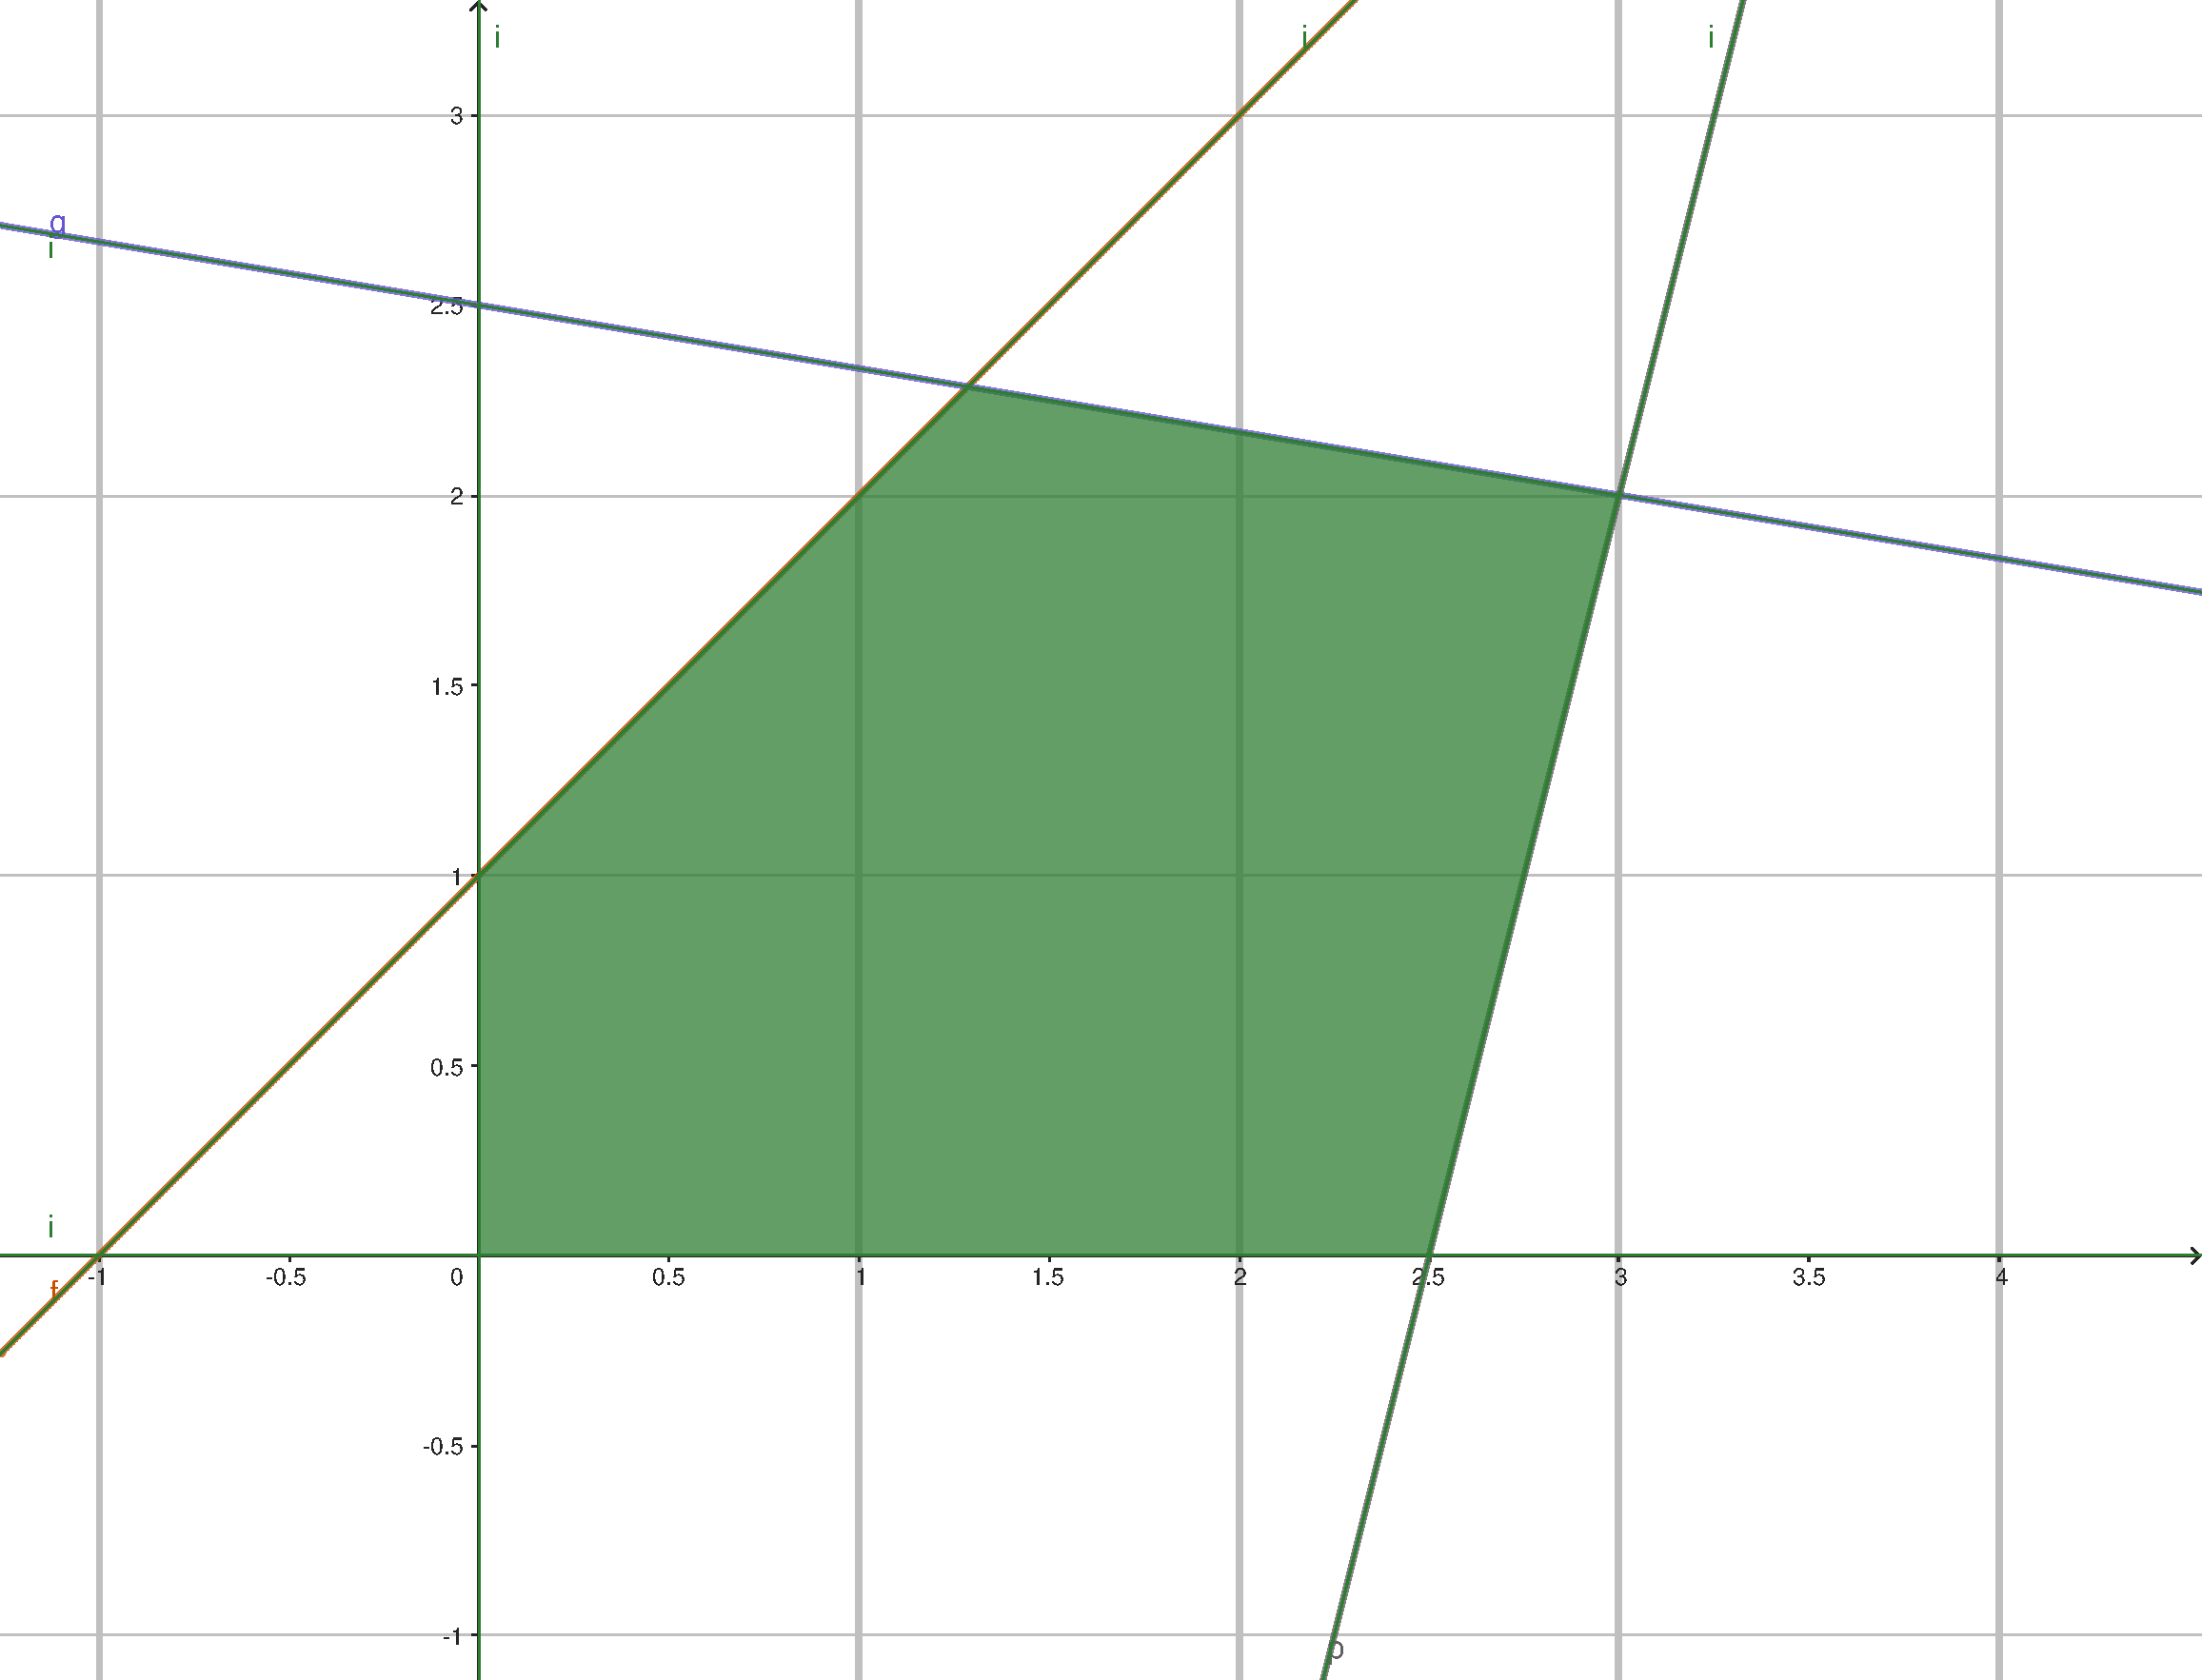
\includegraphics[width=0.4\textwidth ]{images/LP_esempio1.pdf}
        \caption{Insieme dei punti ammissibili}
        \label{LP_esempio1}
    }
\end{figure}
La funzione obiettivo essendo lineare si può rappresentare come prodotto scalare fra due vettori $\mathbf c$ e $\mathbf x$ 
$$\mathbf c^T\mathbf x=\begin{bmatrix}
    1&1
\end{bmatrix}\begin{bmatrix}
    x_1\\ x_2
\end{bmatrix} =x_1+x_2$$
Può risultare utile rappresentare sul piano anche il vettore $\mathbf c$ e la retta equivalente al sottospazio $$\text{span}(\mathbf c)=\{\alpha \mathbf c \ | \ \alpha \in \R\}$$
\begin{figure}[h]
    \centering{
        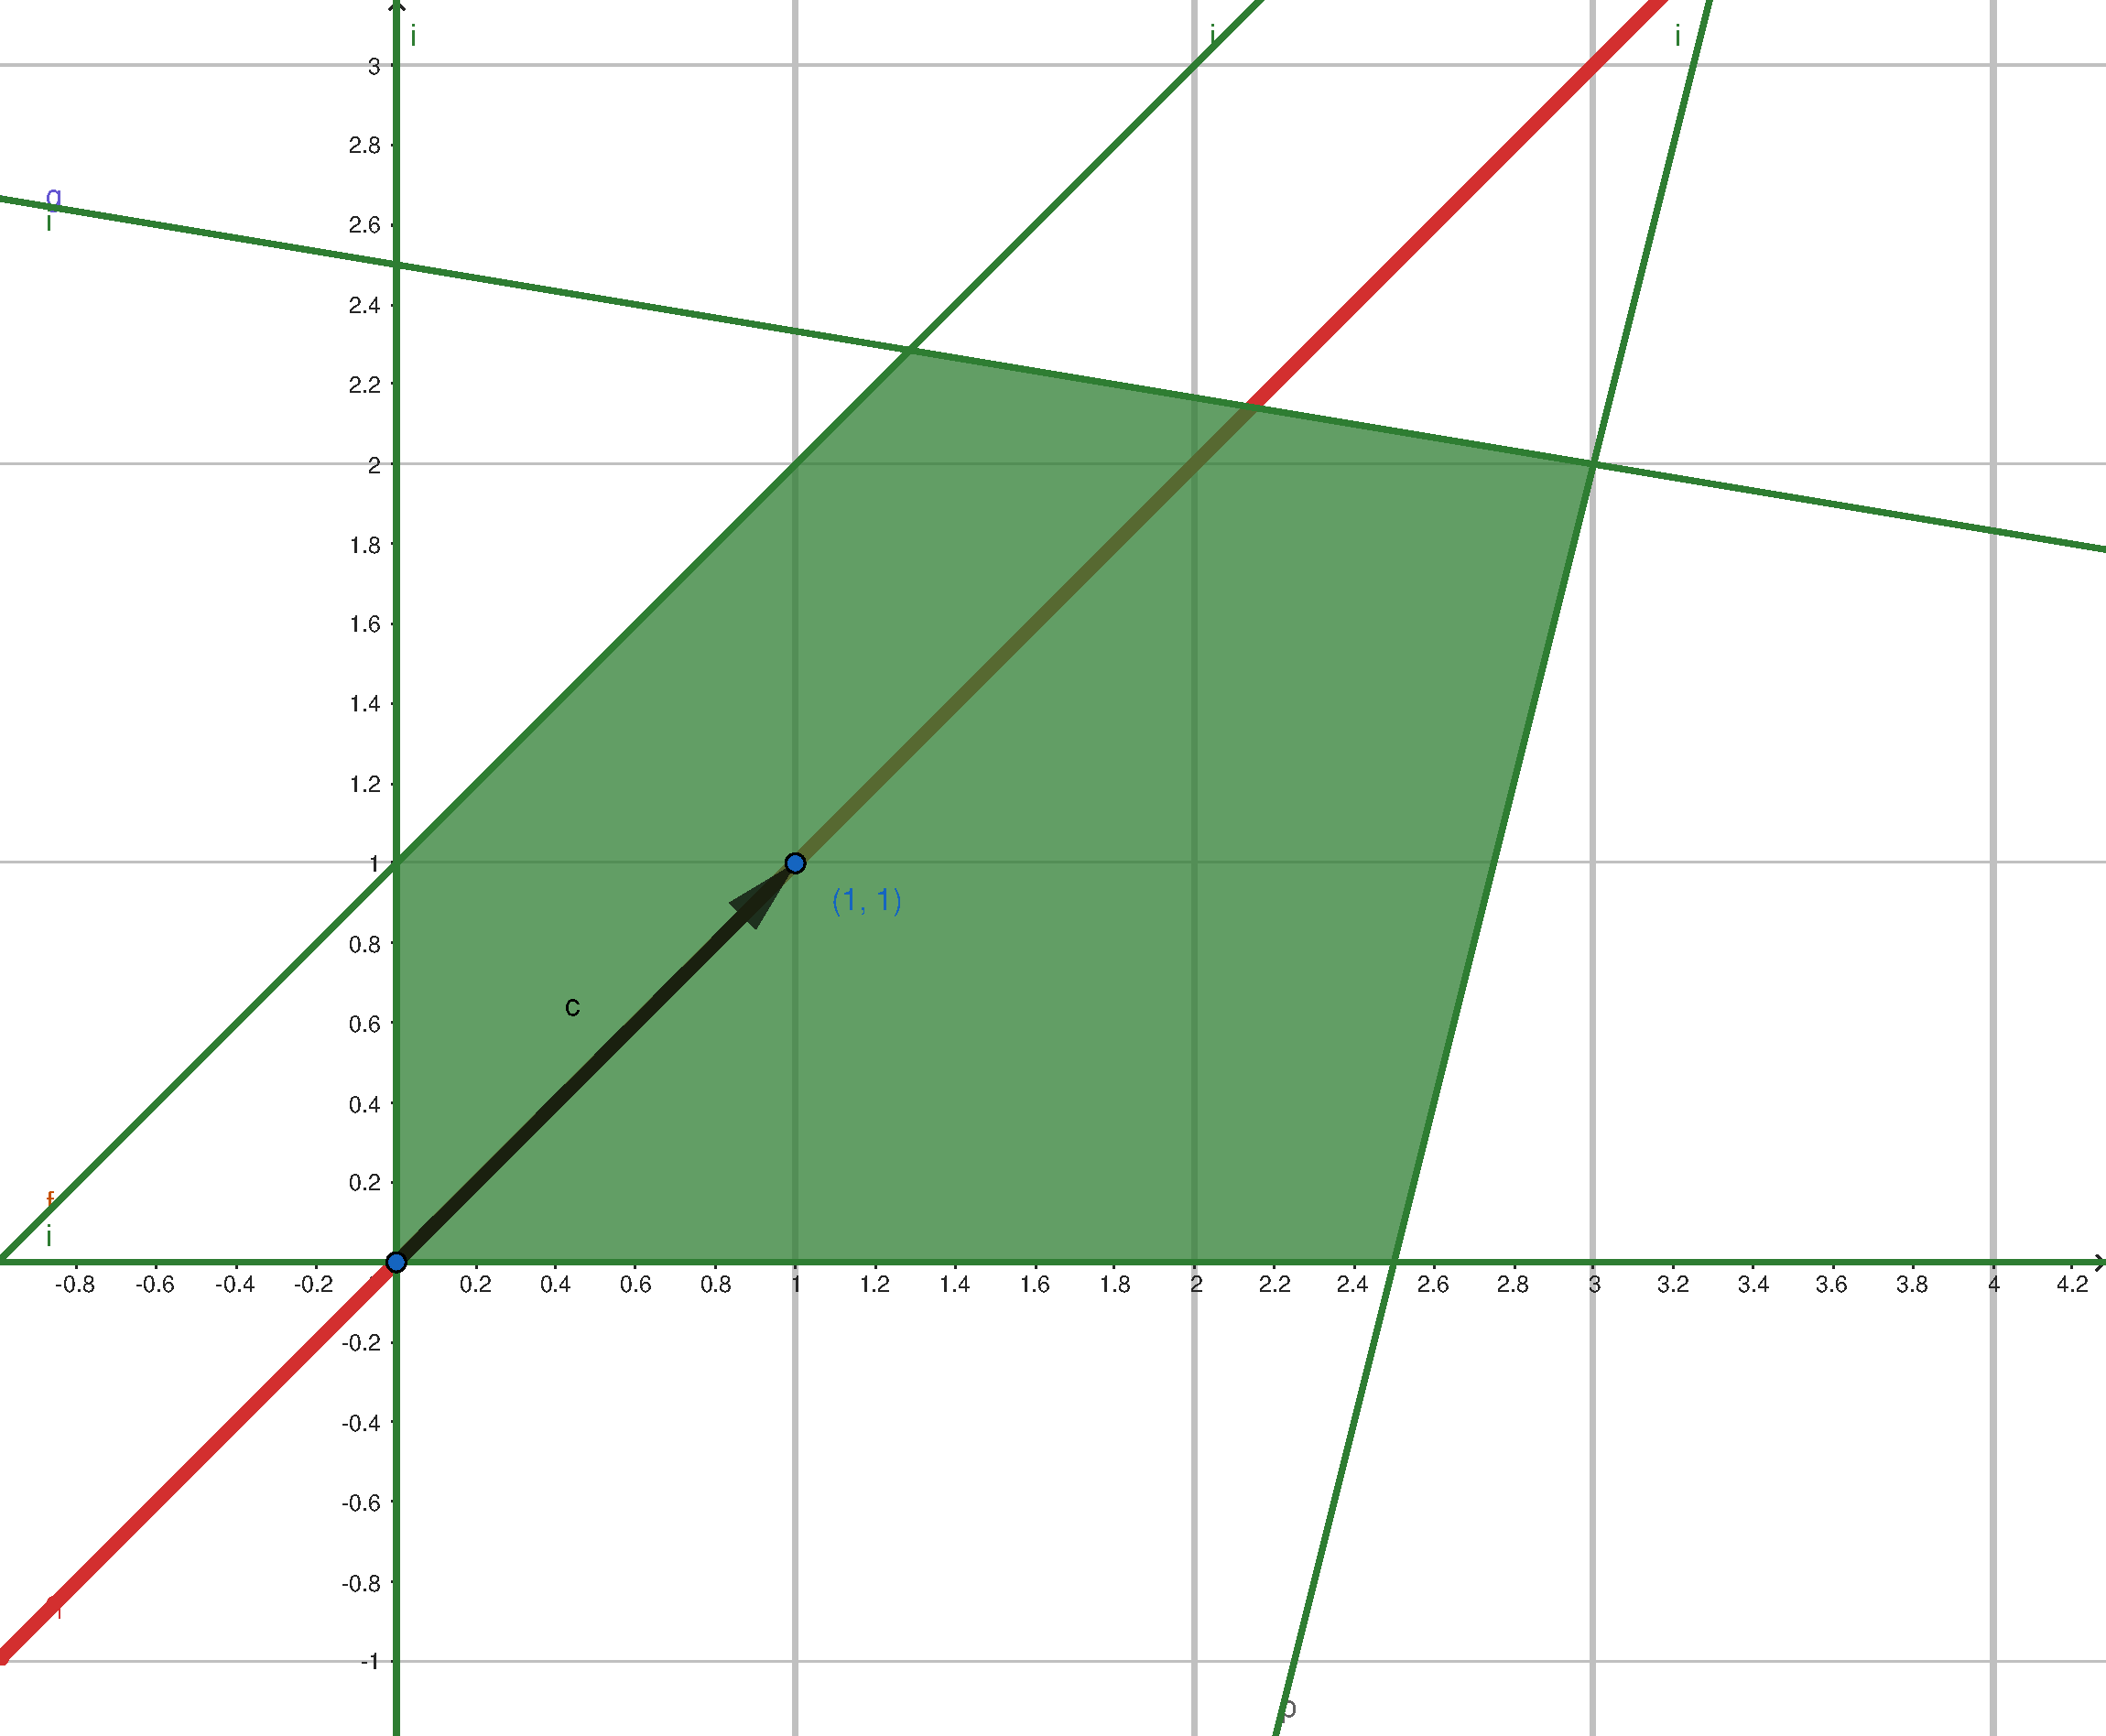
\includegraphics[width=0.4\textwidth ]{images/LP_esempio2.pdf}
    }
\end{figure}
Si consideri una retta $y'$ perpendicolare alla retta definita da $\text{span}(\mathbf c)$, i punti di $y'$ che intersecano l'insieme delle soluzioni ammissibili condividono la stessa immagine se valutati sulla funzione obiettivo. Un'interpretazione geometrica del problema può essere la seguente\begin{quotation}
    Massimizzare la funzione obiettivo equivale a trovare il massimo $\beta$ tale che l'iperpiano definito da $\mathbf c^T\mathbf x = \beta$ perpendicolare alla retta $\alpha \mathbf c$ interseca l'insieme dei punti ammissibili.
\end{quotation}
Si definisce \textbf{soluzione ottimale} ogni soluzione ammissibile che massimizza la funzione obiettivo.
\begin{figure}[h]
    \centering{
        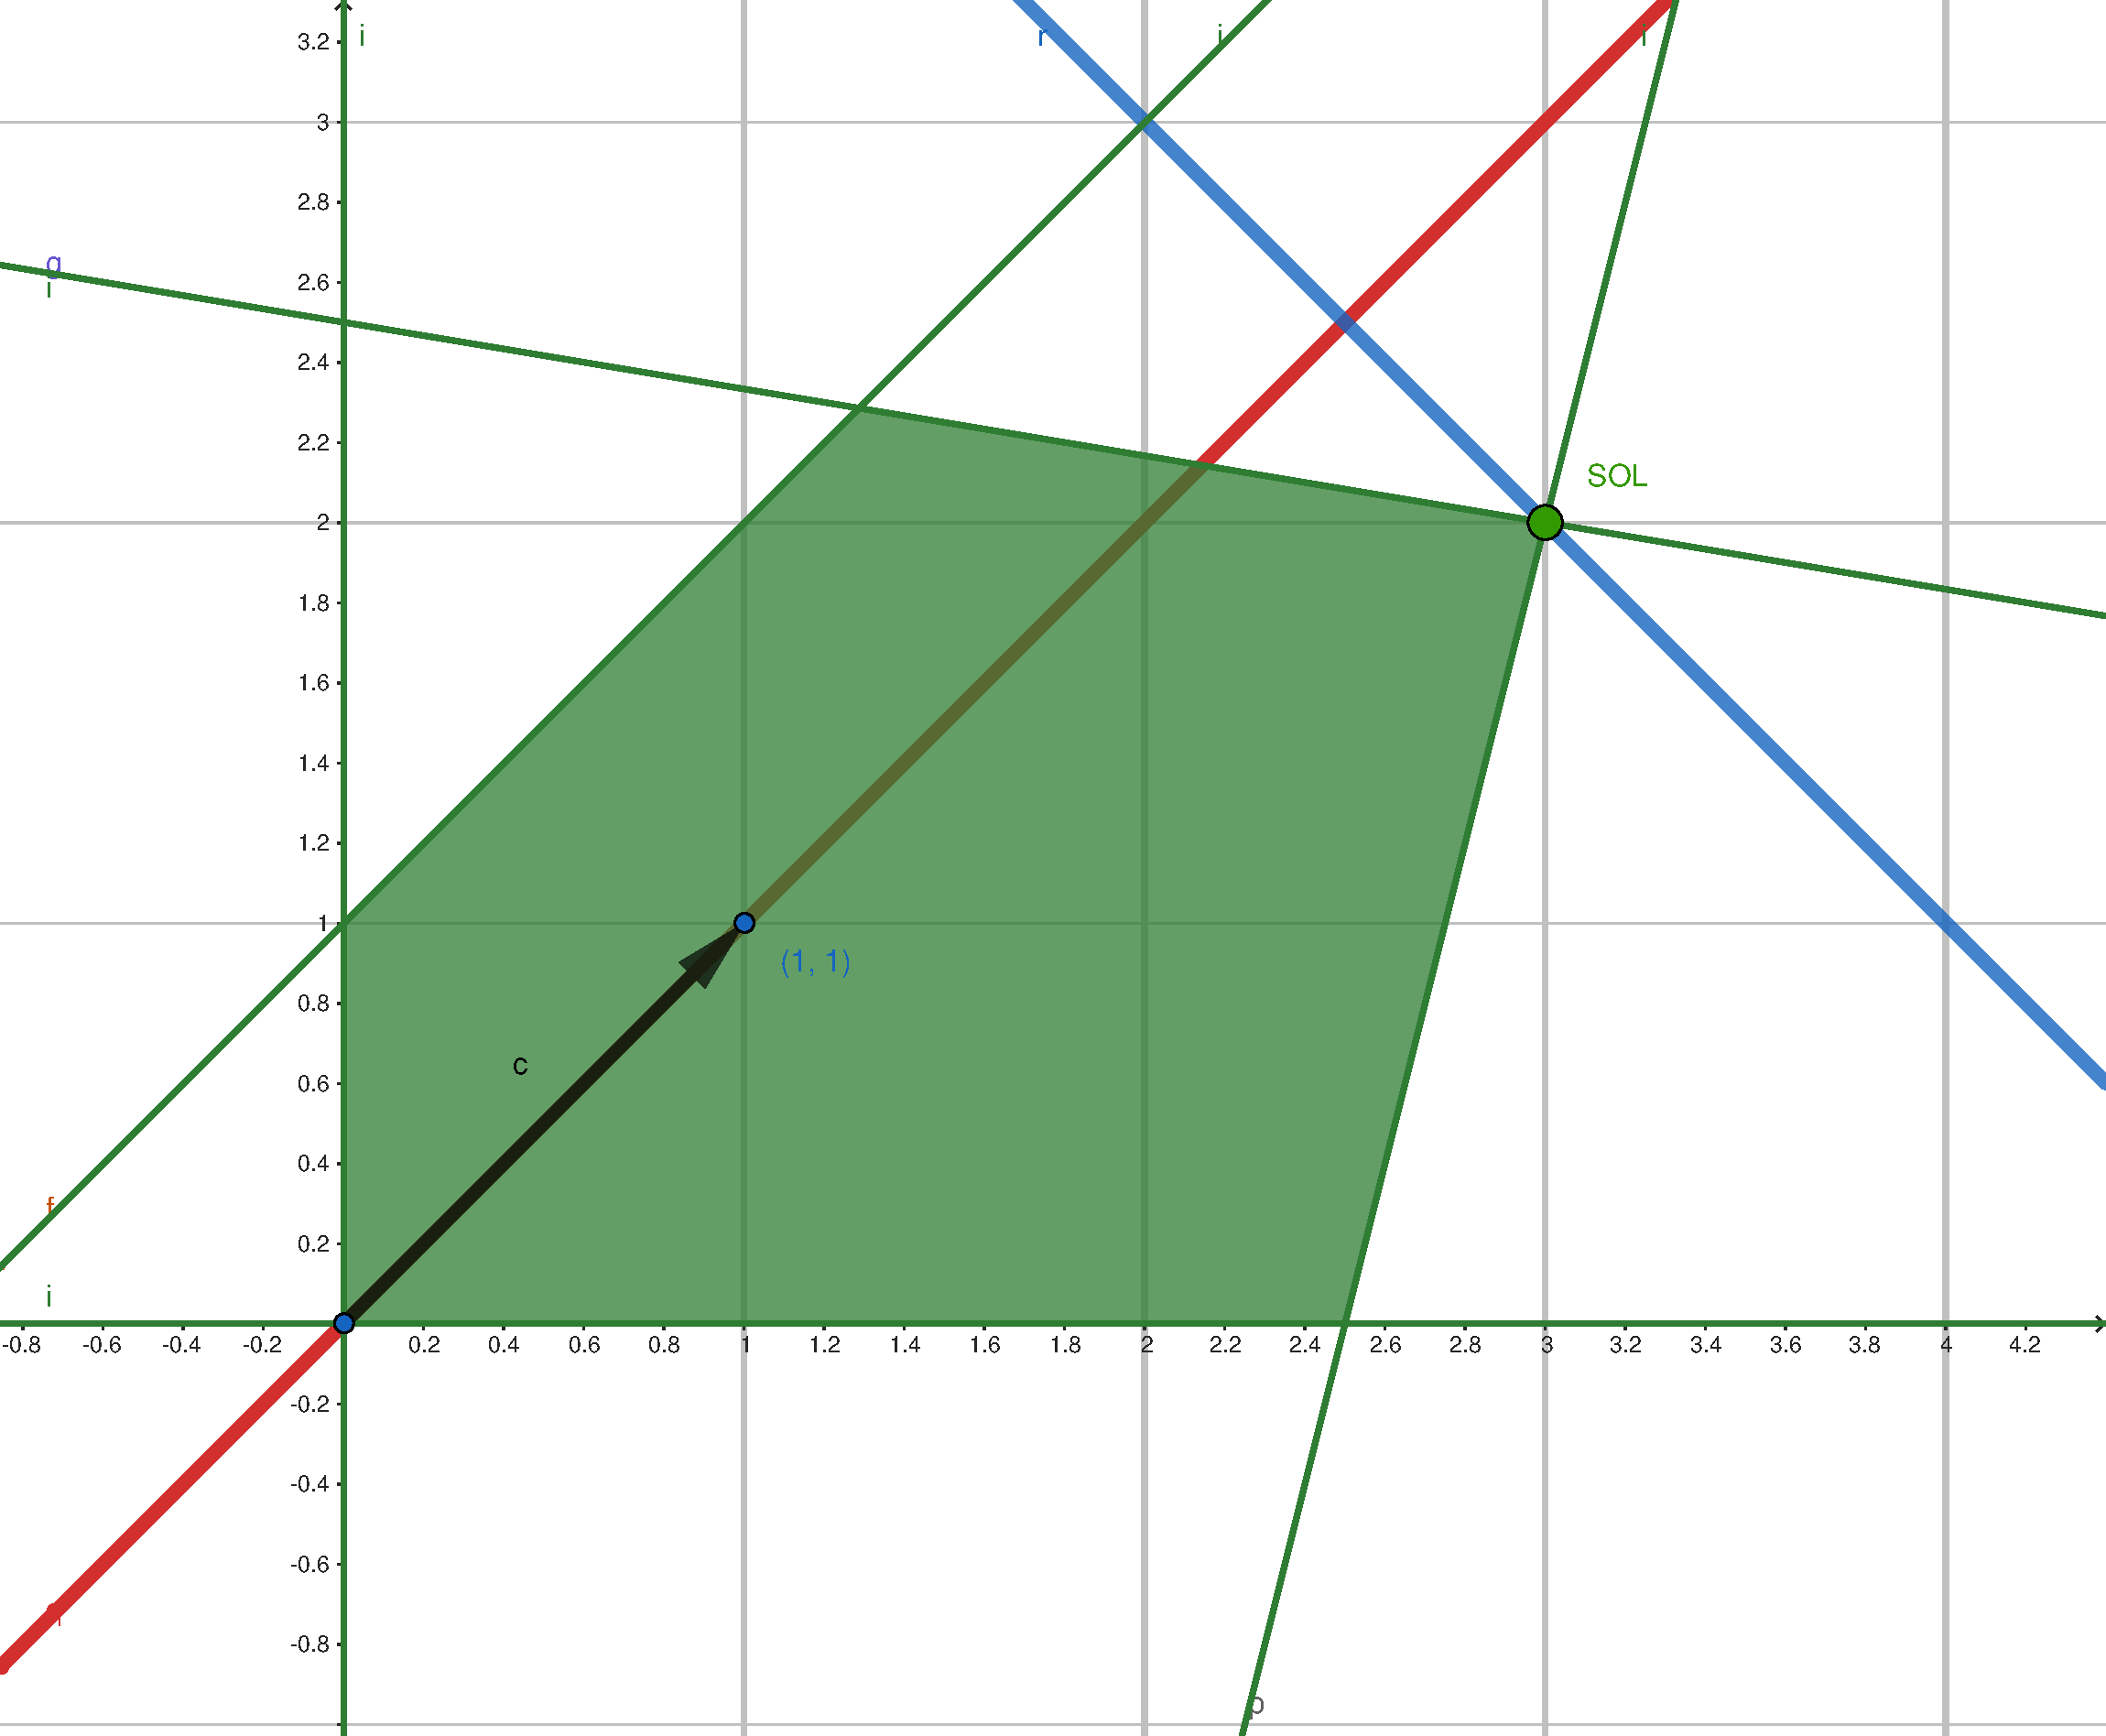
\includegraphics[width=0.4\textwidth ]{images/LP_esempio3.pdf}
    }
    \caption{Il punto $(3,2)$ è una soluzione ottimale per il programma lineare}
        \label{LP_esempio3}
\end{figure}
Il numero di soluzioni di un programma lineare può variare fra i seguenti casi\begin{enumerate}
    \item Vi è un'unica soluzione ottimale.
    \item Vi sono infinite soluzioni ottimale.
    \item Non ci sono soluzioni ammissibili, nessun punto soddisfa tutti i vincoli lineari.
    \item Non ci sono soluzioni ottimali perché il problema non è limitato, ciò avviene se l'insieme dei punti ammissibili non è chiuso.
\end{enumerate}
Generalmente la funzione obiettivo  $f:\R^n\rightarrow \R$ è del tipo 
$$c_1x_1+c_2x_2+\dots+c_nx_n $$
e gli $m$ vincoli sono della forma $$\begin{matrix}
    a_{11}x_1+a_{21}x_2+\dots + a_{n1}x_2\le b_1\\ 
    a_{12}x_1+a_{22}x_2+\dots + a_{n2}x_2\le b_2\\ \vdots \\ 
    a_{1m}x_1+a_{2m}x_2+\dots + a_{nm}x_2\le b_m
\end{matrix}$$
\begin{osservazione}
    Massimizzare  $\mathbf c^T \mathbf x$ equivale a minimizzare $\mathbf -\mathbf c^T\mathbf x $.
\end{osservazione}
Si può quindi assumere che un generico problema di programmazione lineare riguardi la massimizzazione di una funzione del tipo $\mathbf c^T \mathbf x$ per un fissato $\mathbf c \in \R^n$. Inoltre, ogni vincolo del tipo 
\begin{equation}\label{vincolo} a_{1i}x_1+a_{2i}x_2+\dots + a_{ni}x_n\le b_i\end{equation}
è soddisfatto dagli stessi punti che soddisfano 
$$ -a_{1i}x_1-a_{2i}x_2-\dots - a_{ni}x_2\ge b_i $$
Quindi si può assumere che ogni vincolo sia scritto nella forma \ref{vincolo}. Inoltre ogni vincolo di uguaglianza equivale a due disuguaglianze. Date le precedenti osservazioni, si può definire un'insieme di $m$ vincoli in maniera compatta tramite una matrice $m\times n $ ed un vettore $\mathbf b\in \R^m$. 
$$ A\mathbf x \le \mathbf b$$ 
Inoltre ogni vincolo di positività del tipo $x_i\ge 0$ equivale ad il vincolo $-x_i\le 0$. Se in un programma lineare una variabile $x_i$ può assumere qualsiasi valore in $\R$, si può sostituire con la differenza di due nuove variabili 
$$x_i=z_i-z_i' $$
ed imporre i vincoli $$ z_i,z_i'\ge 0$$ 
in tal modo è possibile, per ogni variabile del programma lineare, imporre la positività. Ciò è utile per definire una \textit{forma standard} per un programma lineare. 
\begin{definizione}\label{formaStandard}
    Un programma lineare in \textbf{forma standard} è un problema di ottimizzazione del tipo 
\end{definizione}
    $$
    \begin{matrix}
        \text{max } \ \mathbf c^T\mathbf x\\ 
        A\mathbf x \le \mathbf b\\ 
        \mathbf x \ge 0
    \end{matrix}
    $$
Dove 
$$ 
\begin{matrix}
    \mathbf x,\mathbf c\in \R^n\\ 
    A \in \text{Mat}(m\times n)\\ 
    \mathbf b\in \R^m
\end{matrix}
$$
L'esistenza di soluzioni ammissibili dipende esclusivamente dalla matrice $A$. È impossibile che un programma lineare abbia un numero finito di soluzioni diverso da 0 e 1. In seguito verrà dimostrato che se un programma lineare ha due punti ammissibili che sono soluzione, allora ha infinite soluzioni.
\begin{definizione}
    Dati due punti $\mathbf x,\mathbf y \in \R^n$, si definisce \textbf{segmento di linea} fra i punti l'insieme \end{definizione} 
    $$ \{\alpha\mathbf x +(1-\alpha)\mathbf y \text{ t.c. }\alpha \in [0,1] \}$$
\begin{definizione}
    Un sotto-insieme $X\subseteq \R^n$ è \textbf{convesso} se la seguente è verificata 
\end{definizione}
$$\forall \mathbf x,\mathbf y \in X, \ \ \  
\{\alpha\mathbf x +(1-\alpha)\mathbf y \text{ t.c. }\alpha \in [0,1] \}\subseteq X
$$
\begin{figure}[h]
    \centering{
        \includegraphics[width=0.7\textwidth ]{images/insiemeConvesso.eps}
    }
\end{figure}
\begin{proposizione}
    L'insieme dei punti ammissibili di un programma lineare è convesso.
\end{proposizione}
\textit{Dimostrazione} : Siano $\mathbf x,\mathbf y\in \R^n$ due punti ammissibili, sia $\alpha\in[0,1]$ fissato, si considera il punto (appartenente al segmento) 
$$\alpha\mathbf x +(1-\alpha)\mathbf y $$ 
si ha che \begin{eqnarray}
    A(\alpha\mathbf x +(1-\alpha)\mathbf y)=\\ 
    \alpha A \mathbf x + (1-\alpha)A\mathbf y = \\ 
    \alpha \mathbf b + (1-\alpha )\mathbf b = \mathbf b 
\end{eqnarray}
quindi Il punto soddisfa gli $m$ vincoli
$$A(\alpha\mathbf x +(1-\alpha)\mathbf y)\le \mathbf b $$
Inoltre essendo che 
$$ \alpha \ge 0, \mathbf x \ge 0, \mathbf y \ge 0$$
si ha che 
$$ \alpha\mathbf x +(1-\alpha)\mathbf y\ge 0$$
Quindi $\alpha\mathbf x +(1-\alpha)\mathbf y$ soddisfa tutti i vincoli del programma lineare, ed appartiene quindi ai punti ammissibili.
\hfill$\blacksquare$
\begin{proposizione}
    Se per un programma lineare esistono due soluzioni ottimali distinte $\mathbf x^*,\mathbf y^*\in \R^n$, allora tale programma lineare ha infinite soluzioni ottimali.
\end{proposizione}
\textit{Dimostrazione} : Sia $ \mathbf z$ un punto sul segmento delineato da $\mathbf x^*,\mathbf y^*$
$$\mathbf z = \alpha\mathbf x^* +(1-\alpha)\mathbf y^* \ \ \text{ per qualche }\alpha \in [0,1] $$
si ha che 
 \begin{eqnarray}
    \mathbf c^T \mathbf z = \\
    \mathbf c^T(\alpha\mathbf x^*  +(1-\alpha)\mathbf y^*)=\\
    \alpha\mathbf c^T\mathbf x^*  +(1-\alpha)\mathbf c^T\mathbf y^*
\end{eqnarray}
Essendo che $\mathbf x^*$ e $\mathbf y^*$ sono entrambe soluzioni ottimali, si ha che $c^T\mathbf x^*=c^T\mathbf y^*$
\begin{eqnarray}
    \alpha\mathbf c^T\mathbf x^*  +(1-\alpha)\mathbf c^T\mathbf y^*=\\ 
    \alpha\mathbf c^T\mathbf x^*  +(1-\alpha)\mathbf c^T\mathbf x^*=
    c^T\mathbf x^*
\end{eqnarray}
Quindi anche $\mathbf z$ è soluzione, essendo che quest'ultimo è un generico punto sul segmento, tutti i punti del segmento sono soluzioni.\hfill$\blacksquare$
\section{Applicazioni della Programmazione Lineare}
Un classico esempio di applicazione riguarda la scelta di una dieta che soddisfi dei vincoli nutrizionali minimizzando il costo degli alimenti. Vi è un'insieme di $n$ alimenti $x_1\dots,x_n$ ed ognuno di questi ha un costo $c_i$, si vuole minimizzare 
$$\sum_{i=1}^nc_ix_i $$
tenendo conto dei vincoli nutrizionali del tipo 
$$ a_{1i}x_1+a_{2i}x_2+\dots + a_{ni}x_n\ge b_i$$
Un'altro esempio riguarda la ricerca di un flusso ottimale per una network $G=(V,E,c,s,t)$, per ogni arco $(i,j)$ vi sarà una variabile $x_{ij}$ che rappresenta il flusso su tale arco, si vuole massimizzare la somma del flusso uscente dal vertice source  $s$
$$ \sum_{(s,j)\in E(G)}x_{sj}$$
I vincoli riguardano la skew simmetria, la conservazione del flusso e il vincolo delle capacità, ad esempio:
$$ \begin{matrix}
    x_{ij}\le c_{ij} \\ 
    x_{ij}=-x_{ji}
\end{matrix}$$
Un'esempio interessante di problema che si riconduce alla programmazione lineare riguarda la ricerca del cerchio di raggio massimo che può essere inscritto in un poligono.
\begin{figure}[h]
    \centering{
        \includegraphics[width=0.3\textwidth ]{images/cerchioPoligono.eps}
    }
\end{figure}
Si assume che i lati del poligono possono essere descritti da un'insieme di rette del tipo $y=mx+b$ con $m\ne 0$.\bigskip 

Si consideri una delle rette $y=mx+b$, si vuole trovare una retta perpendicolare a questa passante per un fissato punto $(x_0,y_0)$. Questa ha equazione 
$$y=\frac{y_0-x}{m}+y_0 $$
Il punto di intersezione è $P=(x',y')$ dove 
\begin{eqnarray}
    x'=\frac{x_0+my_0}{m^2+1}-mb\\ 
    y'=m\frac{x_0+my_0-mb}{m^2+1}+b
\end{eqnarray}
\begin{figure}[h]
    \centering{
        \includegraphics[width=0.35\textwidth ]{images/rettaPassante.eps}
    }
    \caption{retta perpendicolare passante per $(x_0,y_0)$}
\end{figure}
La distanza fra $P$ e $(x_0,y_0)$, applicando la norma euclidea, risulta essere 
\begin{itemize}
    \item $\displaystyle\frac{b+mx_0-y_0}{\sqrt{1+m^2}}$ se $(x_0,y_0)$ si trova sotto la retta 
    \item $\displaystyle\frac{-b-mx_0+y_0}{\sqrt{1+m^2}}$ se $(x_0,y_0)$ si trova sopra la retta 
\end{itemize}
Il programma lineare riguarda la ricerca di un cerchio che massimizzi il raggio $r$ (distanza fra $(x_0,y_0)$ e $P$) variando fra il possibile centro $(x_0,y_0)$ all'interno del poligono, rispettando i vincoli del tipo 
\begin{itemize}
     \item$\frac{b_l+mx_0-y_0}{\sqrt{1+m^2}}\ge r, \ \ \forall  l \in {1,\dots k}$
     \item$\frac{-b_l-mx_0+y_0}{\sqrt{1+m^2}}\ge r\ \ \forall l \in {k+1,\dots n}$
\end{itemize} 
\section{Il Metodo del Simplesso}
Il metodo del simplesso è un'algoritmo per la risoluzione dei programmi lineari. Questi devono però assumere una forma differente da quella standard introdotta nella definizione \ref{formaStandard}. Un programma lineare è definito come segue 
$$
    \begin{matrix}
        \text{max } \ \mathbf c^T\mathbf x\\ 
        A\mathbf x \le \mathbf b\\ 
        \mathbf x \ge 0
    \end{matrix}
    $$
Per ogni generica disuguaglianza del tipo 
$$ a_{1i}x_1+a_{2i}x_2+\dots + a_{ni}x_n\le b_i$$
Si considera una nuova variabile $y_i\ge 0$ detta \textbf{slack}, e la disuguaglianza diventa un'uguaglianza come segue 
$$ a_{1i}x_1+a_{2i}x_2+\dots + a_{ni}x_n+y_i = b_i$$
Vi sarà quindi un vettore $\mathbf y \in \R^m$ che viene introdotto nel problema, che assume la seguente forma 
$$
    \begin{matrix}
        \text{max } \ [\mathbf c^T \ | \ 0 \ \dots \  0]\begin{bmatrix}
            \mathbf x \\\mathbf y
        \end{bmatrix}\\ 
        [A \ | \ \text{Id}_m]\begin{bmatrix}
            \mathbf x \\ \mathbf y
        \end{bmatrix} = \mathbf b\\ 
        \begin{bmatrix}
            \mathbf x \\ \mathbf y
        \end{bmatrix} \ge 0
    \end{matrix}
    $$
Dove Id$_m$ è la matrice identità $m\times m$. Un problema LP di questo tipo è detto in \textbf{forma di equazione}, ed il metodo del simplesso opera su un programma lineare di tale forma. In generale, si scrive 
$$
    \begin{matrix}
        \text{max } \ \mathbf c^T\mathbf x\\ 
        A\mathbf x = \mathbf b\\ 
        \mathbf x \ge 0
    \end{matrix}
    $$
\textbf{Assunzione} : Il programma lineare considerato ha almeno una soluzione ammissibile. Ossia $\exists \bar{\mathbf x}$ tale che $A\bar{\mathbf x}=\mathbf b$ e $\mathbf x \ge 0$. Data la matrice $A$, si considerino due righe di essa, ossia $A_i$ e $A_j$, sia $A'$ un'altra matrice identica a $A$, in cui la riga $j$-esima è sostituita con la riga $A_i+A_j$
\begin{equation}
    A=\begin{bmatrix}
        a_{11}& \dots & a_{1n}\\ 
        \vdots & & \vdots \\ 
        a_{i1}& \dots & a_{in}\\ 
        \vdots & & \vdots \\ 
        a_{j1}& \dots & a_{jn}\\ 
        \vdots & & \vdots \\ 
        a_{m1}& \dots & a_{mn}
    \end{bmatrix} \ \ \ \ \ \ \  A'=\begin{bmatrix}
        a_{11}& \dots & a_{1n}\\ 
        \vdots & & \vdots \\ 
        a_{i1}& \dots & a_{in}\\ 
        \vdots & & \vdots \\ 
        a_{j1}+a_{i1}& \dots & a_{jn}+a_{in}\\ 
        \vdots & & \vdots \\ 
        a_{m1}& \dots & a_{mn}
    \end{bmatrix}
\end{equation}
Se $\mathbf x$ soddisfa $A\mathbf x = \mathbf b$ allora soddisfa anche $A'\mathbf x = \mathbf b'$ dove $\mathbf b'$ è identico a $\mathbf b$ ma il $j$-esimo elemento è sommato all'$i$-esimo $$ \mathbf b' = [b_1 \ \ \dots b_i \ \ \dots \ \ b_i+b_j \ \ \dots b_n]^T$$
Le operazioni sulle righe di $A$ non cambiano l'insieme delle soluzioni, si assume che le righe siano \textit{linearmente indipendenti}, che il rango di $A$ sia $m$, e che lo span delle righe di $A$ è un sottospazio di $\mathbb{R}^n$.\begin{proposizione}
    Il rango delle colonne di $A$ è $m$, la dimensione del sottospazio di $\mathbb R^m$ dato dallo span delle colonne è $m$.
\end{proposizione}
\textit{Dimostrazione} : \redText{TODO}\bigskip 

Il problema descritto è \begin{eqnarray}
    A\mathbf x = \mathbf b \\ \mathbf x \ge 0 \\ \text{esiste una soluzione}\\ 
    \text{rango righe di }A=\text{rango colonne di }A=m
\end{eqnarray}
Considerando $\ker(A)=\{\mathbf x \text{ t.c. }A\mathbf x = \mathbf 0\}$ si ha un sottospazio di dimensione $n-m$ di $\mathbb R^n$, lo spazio delle soluzioni di $A\mathbf x = \mathbf b$ è un \textbf{sottospazio affine} e si ottiene sommando $\mathbf b$ a tutti i vettori di $\ker(A)$.\bigskip 
\subsection{Soluzioni Ammissibili Basiche}
\textit{Esempio} : Si consideri il triangolo delineato dai punti $(0,0,3),(0,3,0),(3,0,0)$, tutti i punti di tale triangolo sono i vettori $\mathbf x$ che soddisfano $A\mathbf x = \mathbf b$.\begin{figure}[h]
    \centering{
        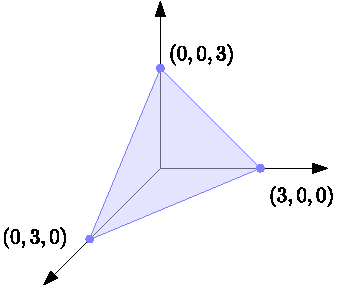
\includegraphics[width=0.35\textwidth ]{images/triangolo.pdf}
    }
    \caption{triangolo in $\mathbb R^3$}
\end{figure}
Si ha $A=[1 \ \ 1 \ \ 1]$ e $b=3$
$$ \begin{bmatrix}
    1 & 1 & 1
\end{bmatrix}\begin{bmatrix}
    x \\ y \\ z
\end{bmatrix}=3\implies x+y+z=3$$
I 3 vertici del triangolo rappresentano delle soluzioni "speciali", ottenute ponendo 2 delle 3 variabili uguali a zero e risolvendo per le altre, tali soluzioni sono dette \textit{basiche}.\bigskip 

In generale, $A\in Mat(m\times n)$ e $\mathbf b \in \mathbb R^n$, si vogliono porre un numero massimale di variabili pari a zero e risolvere per le altre, si pongono esattamente $n-m$ variabili nulle. 

Sia $\mathcal B \subseteq \{1,\dots n\}$ l'insieme degli indici $i$ per cui la variabile $x_i$ non è posta a zero, e sia $A_{\mathcal B}$ la sotto-matrice di $A$ composta dalle colonne il cui indice è relativo ad una variabile diversa da zero.
$$ \begin{bmatrix}
    a_{1i} & \dots & a_{mi}
\end{bmatrix}^T \text{ è una colonna di }A_{\mathcal B} \iff i\in\mathcal B$$
Sia $\mathbf b_{\mathcal B}$ definito in maniera intuitiva, come il vettore contenente la componente $j$-esima di $\mathbf b$ se $j\in \mathcal B$. Si considera il problema derivato \begin{equation}
    A_{\mathcal B}\mathbf x_{\mathcal B}=\mathbf b_{\mathcal B} \ \ \ \ A_{\mathcal{B}}\in Mat(m\times m)
\end{equation}
Se $A_{\mathcal{B}}$ non è \textbf{singolare} (il determinante è diverso da zero) allora esiste una soluzione $\bar{ \mathbf x}$ per il problema derivato, se $\bar{ \mathbf x}\ge 0$, allora è anche una soluzione per il problema originale, ponendo a zero tutte le componenti della soluzione i cui indici non sono in $\mathcal B$.\begin{itemize}
    \item se $\bar{ \mathbf x}=[x_{k1} \ \ x_{k2} \ \ \dots \ \ x_{km}]^T$ è soluzione di  $ A_{\mathcal B}\mathbf x_{\mathcal B}=\mathbf b_{\mathcal B}$
    \item si ha $\{k1,k2\dots, km\}=\mathcal B$
    \item allora il vettore $\bar{ \mathbf x}'$ con\begin{itemize}
        \item $x_i = x_{kj}$ se $i=kj$ per qualche $j\le m$, ossia $i\in\mathcal B$
        \item $x_i = 0 $ se $i \notin \mathcal B$
    \end{itemize}
    è soluzione di $A\mathbf x = \mathbf b$ se $\bar{ \mathbf x}'\ge 0$.
\end{itemize}
\begin{definizione}
    Dato un programma lineare $$
    \begin{matrix}
        \text{max } \ \mathbf c^T\mathbf x\\ 
        A\mathbf x \le \mathbf b\\ 
        \mathbf x \ge 0
    \end{matrix}
    $$
    Una soluzione ammissibile $\bar{\mathbf x}$ è detta \textbf{basica} (BFS) se esiste un sotto-insieme di indici $\mathcal B\subseteq \{1,2,\dots n\}$ tale per cui\begin{itemize}
        \item $A_{\mathcal B}$ non è singolare 
        \item $\bar{x}_j=0$ $\forall j \notin \mathcal{B}$
    \end{itemize}
\end{definizione}
\textit{Esempio} : Data la matrice \begin{equation}
    A=\begin{bmatrix}
        1&6&3&-3&4\\ 
        0&1&3&2&4
    \end{bmatrix}
\end{equation}
Ed il sistema di equazioni 
$$ A\mathbf x = \begin{bmatrix}
    6\\6
\end{bmatrix}$$
Per la base  $\mathcal B = \{2,4\}$ si ha $$A_{\mathcal B}=\begin{bmatrix}
    6&-3\\1&2
\end{bmatrix} $$
La matrice non è singolare, per il sistema $$ \begin{bmatrix}
    6&-3\\1&2
\end{bmatrix}\begin{bmatrix}
    x_2\\x_4
\end{bmatrix}  = \begin{bmatrix}
    6\\6
\end{bmatrix}$$
una soluzione è $$ \begin{bmatrix}
    2\\2
\end{bmatrix}$$
Quindi una soluzione ammissibile basica per il problema originale è 
$$ \bar{\mathbf x}=\begin{bmatrix}
    0&2&0&2&0
\end{bmatrix}^T$$
Se considerassimo la base $\mathcal B' = \{3,5\}$, si avrebbe la sotto-matrice 
$$A_{\mathcal B'}= \begin{bmatrix}
    3&4\\3&4
\end{bmatrix}$$
Essendo singolare, per tale base non esiste alcuna soluzione basica.
\begin{proposizione}\label{insiemeK}
    Sia $A\mathbf x=b$, $\mathbf x \ge 0$ un programma lineare, e sia $\mathbf{\bar x}$ una BFS (soluzione ammissibile basica), si consideri l'insieme di indici 
    $$ K=\{i \text{ t.c. }\bar x_i>0\}$$
    Le colonne della matrice $A_K$ sono linearmente indipendenti. 
\end{proposizione}
\textit{Dimostrazione} : La dimostrazione è banale, esiste una base $\mathcal B$ a cui $\mathbf{\bar x}$ fa riferimento per cui $K\subseteq \mathcal B$, essendo le colonne di $A_{\mathcal B}$ linearmente indipendenti, anche un loro sotto-insieme, ossia quelle di $A_K$ lo sono.\hfill$\blacksquare$
\begin{proposizione}
    Si consideri un programma lineare, sia $\mathbf{\bar x}$ una soluzione ammissibile e $$ K=\{i \text{ t.c. }\bar x_i>0\}$$ $\mathbf{\bar x}$ è una BFS se e solo se le colonne di $A_K$ sono linearmente indipendenti.
\end{proposizione}
\textit{Dimostrazione} : Verrà dimostrata solo una delle due implicazioni, si assume che $\mathbf{\bar x}$ è una soluzione ammissibile e che le colonne di $A_K$ siano linearmente indipendenti. Per dimostrare che $\mathbf{\bar x}$ sia una BFS è necessario trovare una base che contenga $K$.

Sia $\mathcal B^*$ un'insieme definito come segue\begin{enumerate}
    \item $K\subseteq\mathcal B^*$
    \item Le colonne di $\mathcal B^*$ sono linearmente indipendenti 
    \item $\mathcal B^*$ è l'insieme massimale che rispetti le due condizioni precedenti
\end{enumerate}
Bisogna mostrare che $\mathcal B^*$ ha $m$ elementi in modo tale che $A_{\mathcal B^*}$ sia una matrice quadrata $m\times m$.

Si assuma che $|\mathcal B^*|<m$, ciò significherebbe che le restanti colonne di $A$ sono contenute nello span delle colonne di $A_{\mathcal B^*}$, quindi $A$ ha \textit{meno} di $m$ colonne linearmente indipendenti, ma è noto che il rango di $A$ sia $m$, quindi l'assunzione  $|\mathcal B^*|<m$ porta ad una contraddizione $\implies |\mathcal B^*|=m$.\hfill$\blacksquare$
\begin{osservazione}
    Ogni base ha almeno una BFS associata.
\end{osservazione}
\textbf{Conclusione} : Esiste un numero finito di BFS. Ogni base è un sotto-insieme di $m$ elementi preso da $\{1,2,\dots n\}$, quindi esistono al più $\binom{n}{m}$ basi distinte, quindi esistono al più $\binom{n}{m}$  BFS.\bigskip 

Il seguente risultato è fondamentale in quanto stabilisce che un programma lineare (che riguarda la ricerca di una soluzione fra un'insieme non numerabile) si può ridurre ad una ricerca fra un'insieme finito di possibili soluzioni ottimali. 
\begin{teorema}\label{teo:BFS}
    Si consideri un programma lineare in forma di equazione
$$ 
\begin{matrix}
    \text{max } \ \mathbf c^T\mathbf x\\ 
    A\mathbf x = \mathbf b\\ 
    \mathbf x \ge 0
\end{matrix}
$$\begin{enumerate}
    \item Se esiste almeno una soluzione ammissibile ed il problema è limitato (l'insieme delle soluzioni ammissibili è compatto), allora esiste una soluzione ottimale.
    \item Se esiste una soluzione ottimale, allora esiste anche una BFS che è a sua volta ottimale.
\end{enumerate}
\end{teorema}
La dimostrazione del teorema \ref{teo:BFS} richiede alcuni passi preliminari. \acc 
\textbf{Statement} $\star$ : Se la funzione obiettivo di un LP in forma di equazione è limitata superiormente, allora per ogni soluzione ammissibile $\mathbf y$ esiste una BFS $\mathbf z$ tale che $\mathbf c^T\mathbf z\ge \mathbf c^T\mathbf y$.\acc 
\textbf{Claim 1} : Se $\star$ è vera, allora il teorema è dimostrato.\acc 
\textit{Dimostrazione Claim 1} : Si consideri la BFS $\mathbf y$ che massimizza la funzione obiettivo rispetto tutte le altre BFS. Assumiamo che $\mathbf y$ non sia ottimale, allora esiste $\mathbf y^*$ (che non è una BFS) tale che 
$$\mathbf c^T\mathbf y^*\ge \mathbf c^T\mathbf y$$
Ma per il claim $\star$ esiste una BFS $\mathbf z$ tale per cui 
$$\mathbf c^T\mathbf z\ge\mathbf c^T\mathbf y^*\ge \mathbf c^T\mathbf y$$
Ciò va in contraddizione con l'assunzione che $\mathbf y$ sia massimale fra le BFS, quindi non può esistere tale $\mathbf y^*\implies \mathbf y$ è una BFS ottimale $\implies$ il claim è dimostrato : $\star \implies $ teorema \ref{teo:BFS}.\hfill$\blacksquare$\bigskip

Per dimostrare il teorema è quindi sufficiente dimostrare lo Statement $\star$.
Sia $\mathbf y$ un'arbitraria soluzione ammissibile, sia $\mathbf z$ un'altra soluzione ammissibile tale che \begin{enumerate}
    \item $\mathbf  c^T\mathbf z\ge \mathbf  c^T\mathbf y$
    \item $\mathbf z$ ha un numero massimale di componenti uguali a zero
\end{enumerate}
Tale $\mathbf z$ esiste dato che nel caso peggiore si può considerare $\mathbf z = \mathbf y$. Si consideri l'insieme $K$ degli indici delle componenti positive di $\mathbf z$ 
$$ K=\{j \text{ t.c. }z_j>0\}$$
La proposizione \ref{insiemeK} afferma che se le colonne di $A_K$ sono linearmente indipendenti $\mathbf z$ è una BFS, ciò dimostrerebbe lo Statement $\star$.

Si assuma  che le colonne di $A_K$ siano linearmente dipendenti. Sia $k=|K|$. Esistono dei coefficienti $\alpha_1\dots, \alpha_k$ tali per cui 
\begin{equation}\label{linDIP}
    \alpha_1\begin{bmatrix}
        \\A^1_K\\ \\
    \end{bmatrix}+\dots + \alpha_k\begin{bmatrix}
        \\A^k_K\\ \\
    \end{bmatrix}=\mathbf 0\implies 
\end{equation}\begin{equation}\label{linDIP2}
    A_K\begin{bmatrix}
        \alpha_1\\\vdots\\\alpha_k 
    \end{bmatrix}=\mathbf 0
\end{equation}
Si consideri un particolare vettore $\mathbf w$ definito come segue\begin{itemize}
    \item la componente $j$-esima di $\mathbf w$ contiene $\alpha_j$ se $j\in K $, $\alpha_j$ è il coefficiente moltiplicato alla colonna $j$-esima di $A_K$ nella combinazione lineare dell'equazione  \ref{linDIP}.
    \item Se $j\notin K$, allora la componente $j$-esima di $\mathbf w$ è 0.
\end{itemize}
Data l'equazione \ref{linDIP2}, risulta chiaro che il prodotto della matrice originale $A$ e $\mathbf w$ sia uguale al prodotto fra $A_K$ ed il vettore dei coefficienti $\alpha_1\dots,\alpha_k$. 
\begin{equation}\label{linDIP3}
   A\mathbf w= A_K\begin{bmatrix}
        \alpha_1\\\vdots\\\alpha_k 
    \end{bmatrix}=\mathbf 0
\end{equation}
Riconsiderando la soluzione $\mathbf z$, si può sommare a $\mathbf w$ e moltiplicare per la matrice $A$ 
$$ A(\mathbf z+\mathbf w)=A\mathbf z+A\mathbf w=A\mathbf z+\mathbf 0 = \mathbf b+\mathbf 0 = \mathbf b$$
Essendo che $\mathbf z$ è soluzione il prodotto fra quest'ultimo ed $A$ è uguale al vettore $\mathbf b$ relativo ai vincoli del programma lineare. Nonostante $\mathbf z+\mathbf w$ soddisfi i vincoli, non è certo che sia soluzione, in quanto non è certo se abbia o no componenti negative (si ricordi che una soluzione deve essere maggiore o uguale al vettore $\mathbf 0$).

Si noti come per definizione di $\mathbf w$, questo ha una componente uguale a zero in una data posizione, se in quella data posizione la soluzione $\mathbf z$ ha la componente uguale a zero, quindi $\mathbf w$ ha \textit{almeno tanti} zeri quanti quelli di $\mathbf z$.\acc 
\textbf{Claim 2} : Il vettore $\mathbf w$ soddisfa le seguenti\begin{enumerate}
    \item $\mathbf c^T\mathbf w \ge 0$
    \item $\exists j\in K \text{ t.c. }w_j<0$
\end{enumerate}
\textit{Dimostrazione} : Se per $\mathbf w$ il punto (2) non dovesse essere soddisfatto, si potrebbe considerare $-\mathbf w$, questo soddisfa tutte le condizioni per cui è stato definito $\mathbf w$ : $A(-\mathbf w)=A\mathbf w =\mathbf 0$. Tale sostituzione si può considerare anche per soddisfare il punto (1), nel caso in cui si dovesse verificare che $c^T\mathbf w<0$.

Se la condizione (2) non dovesse essere soddisfatta, allora si consideri il vettore (in funzione di $t\in\mathbb R^+$)  $$\mathbf z(t)=\mathbf{z}+t\mathbf w$$
Tale vettore soddisfa i vincoli del programma lineare 
$$A\mathbf z(t)=A(\mathbf z + t\mathbf w)=A\mathbf z+tA\mathbf w=\mathbf b + t\cdot \mathbf 0 = \mathbf b $$
Inoltre essendo la (2) non soddisfatta, si ha che, per ogni possibile $t\in\mathbb R^+$ $$ z(t)_j=z_j+tw_j\ge 0$$ questo perché \begin{enumerate}
    \item $z_j\ge 0$ essendo $\mathbf z$ una soluzione 
    \item $t$ è non negativo perché varia in $\mathbb  R^+$
    \item $w_j$ non è negativo dato che la (2) non è soddisfatta
\end{enumerate}
Essendo $\mathbf z(t)$ sempre maggiore o uguale a zero si ha: \begin{equation}
    \mathbf c^T \cdot \mathbf z(t)= \mathbf c^T (\mathbf z + t\mathbf w)=\mathbf c^T \mathbf z + t\mathbf c^T \mathbf w
\end{equation}
Attenzione, essendo il punto (1) soddisfatto, $c^T \mathbf w$ è positivo, quindi dato il termine $t\mathbf c^T \mathbf w$, la funzione $ \mathbf c^T \cdot \mathbf z(t)$ non è limitata, ciò è una contraddizione, quindi le due assunzioni del claim sono vere. \hfill$\blacksquare$\bigskip

Dato ciò, esiste un indice $j\in K$ per cui $w_j<0$, si consideri nuovamente il vettore $$\mathbf z(t)=\mathbf{z}+t\mathbf w$$
Avendo verificato che questo soddisfa i vincoli $\forall t$, ci si pone la domanda, che valore assume nella funzione obiettivo? 
$$ \mathbf c^T \mathbf z(t)=\mathbf c^T\mathbf z+t\mathbf c^T\mathbf w$$
Sappiamo che\begin{itemize}
    \item $\mathbf c^T\mathbf z\ge \mathbf c^T\mathbf y$ per la scelta di $\mathbf z$
    \item $t\mathbf c^T\mathbf w\ge 0$ per il claim
\end{itemize}
Ne consegue che $$ \mathbf c^T \mathbf z(t)\ge \mathbf c^T \mathbf y$$
Per la chiarezza della dimostrazione, si ricordi che $\mathbf z$ è stato scelto per soddisfare le seguenti \begin{enumerate}
    \item $\mathbf  c^T\mathbf z\ge \mathbf  c^T\mathbf y$
    \item $\mathbf z$ ha un numero massimale di componenti uguali a zero
\end{enumerate}
$$ 
\mathbf z(t)=\begin{bmatrix}
    0\\\vdots \\ z_i\\ \vdots \\0
\end{bmatrix}+t\begin{bmatrix}
    0\\\vdots \\ w_i\\ \vdots \\0
\end{bmatrix}
$$
sia $ w_i$ una componente negativa di $\mathbf w$, se $t=-\frac{z_i}{w_i}$ allora 
$$ 
\mathbf z(-\frac{z_i}{w_i})=\begin{bmatrix}
    0\\\vdots \\ z_i\\ \vdots \\0
\end{bmatrix}-\frac{z_i}{w_i}\begin{bmatrix}
    0\\\vdots \\ w_i\\ \vdots \\0
\end{bmatrix}\implies z(-\frac{z_i}{w_i})_i=z_i-z_i=0
$$
Il vettore $\mathbf z(-\frac{z_i}{w_i})$ ha una componente  nulla in più rispetto a $\mathbf z$, se si considera $$ t^*=\min_{i \text{ t.c. }w_i<0}(-\frac{z_i}{w_i})$$
il vettore $\mathbf z(t^*)$ risulterà non negativo, quindi: 
$$\begin{matrix}
    A\mathbf z(t^*=\mathbf b)\\ \mathbf z(t^*)\ge 0
\end{matrix}$$
Il vettore $\mathbf z(t^*)$ è una soluzione ammissibile ed ha uno 0 in più rispetto a $\mathbf z$, ma questa è una contraddizione (data la scelta di $\mathbf z$), quindi è impossibile che le colonne di $A_K$ siano linearmente dipendenti $\implies$ $\mathbf z$ è una BFS, lo Statement $\star$ è dimostrato.\hfill$\blacksquare$\acc 
\textbf{Corollario} : Se un programma lineare ha una funzione obiettivo limitata, allora esiste un'algoritmo che trova una soluzione ottimale in un numero finito di passi.
\subsection{Ricerca sul Poliedro}\label{RicercasulPoliedro} 
Si consideri il seguente programma lineare$$\begin{matrix}
    \max \ x_1+x_2\\ -x_1+x_2\le 1 \\ x_1\le 3 \\ x_2 \le 2 \\ x_1,x_2 \ge 0
\end{matrix}$$
L'insieme delle soluzioni ammissibili è mostrato in figura \ref{fig:solEsempio}.
\begin{figure}[h]\label{fig:solEsempio}
    \centering{
        \includegraphics[width=0.35\textwidth ]{images/insiemeSoluzioniLP1.eps}
    }
    \caption{Insieme definito dai vincoli}
\end{figure}
Per trasformare il problema in forma di equazione occorre aggiungere 3 variabili slack $x_3,x_4,x_5$.$$\begin{matrix}
    \max \mathbf{c}^T \mathbf x  \ \\ -x_1+x_2+x_3= 1 \\ x_1+x_4= 3 \\ x_2 +x_5= 2 \\ x_1,x_2,x_3,x_4,x_5 \ge 0
\end{matrix}$$
in forma matriciale:
$$A=\begin{bmatrix}
    -1&1&1&0&0\\ 
    1&0&0&1&0 \\ 
    0& 1 & 0 & 0 & 1
\end{bmatrix}  \ \ \ \ \mathbf c = \begin{bmatrix}
    1 & 1 & 0&0&0
\end{bmatrix}^T$$
Si consideri la base $\mathcal B = \{1,2,4\}$ : 
$$A_{\mathcal B}=\begin{bmatrix}
    -1&1&0\\ 1&0&1\\0&1&0
\end{bmatrix} 
$$
è non singolare, si può risolvere il sistema di equazioni 
\begin{eqnarray}\begin{bmatrix}
    -1&1&0\\ 1&0&1\\0&1&0
\end{bmatrix} \begin{bmatrix}
    x_1\\x_2\\x_4
\end{bmatrix}=\begin{bmatrix}
    1\\ 3\\ 2
\end{bmatrix}\implies  \begin{cases}
    x_1=1\\x_2=2\\x_4=2
\end{cases}
\end{eqnarray}
La BFS è $\mathbf x = \begin{bmatrix}
    1&2&0&2&0
\end{bmatrix}^T$
Le variabili slack $x_3,x_5$ della soluzione $\mathbf x$ sono poste a zero, ciò significa che tale punto soddisfa i vincoli del problema originale (in forma di uguaglianza), in particolare, soddisfa le eguaglianze del primo e del terzo vincolo $$ \begin{matrix}
    -x_1+x_2= 1 \\ x_2 = 2
\end{matrix}$$ 
Tale punto può essere geometricamente individuato nell'insieme delle soluzioni ammissibili del problema originale, ed equivale al punto su cui si intersecano le due rette che definiscono il primo ed il terzo vincolo, come mostrato in figura \ref{fig:solEsempio2}.
\begin{figure}[h]\label{fig:solEsempio2}
    \centering{
        \includegraphics[width=0.35\textwidth ]{images/insiemeSoluzioniLP2.eps}
    }
    \caption{punto di intersezione}
\end{figure}
\begin{definizione}
    Un'insieme $\mathcal X\subset \mathbb R^n$ è \textbf{aperto} se $\forall \mathbf x\in \mathcal X$, $\exists \epsilon >0$ tale che $\{\mathbf y\in \mathbb R^n \ | \ \|\mathbf y-\mathbf x\|\le \epsilon   \}\subset \mathcal X$.
\end{definizione}
\begin{definizione}
    Un'insieme $\mathcal X\subset \mathbb R^n$ è \textbf{chiuso} se il suo complemento $\mathbb R^n \backslash \mathcal X$ è un'insieme aperto.
\end{definizione}
\begin{osservazione}
    L'unione di due insiemi aperti è un'insieme aperto. L'intersezione di due insiemi chiusi è un'insieme chiuso.
\end{osservazione}
\begin{definizione}
    Dato un sotto-insieme di punti  $I\subset \mathbb R^n$, si definisce il suo \textbf{inviluppo convesso} l'intersezione di tutti i sotto-insiemi convessi di $\mathbb R^n$ contenenti $I$. Alternativamente, si può dire che l'inviluppo convesso di $I$ è il più piccolo insieme convesso contenente $I$.
\end{definizione}
\begin{figure}[h]\label{fig:solEsempio2}
    \centering{
        \includegraphics[width=0.4\textwidth ]{images/inviluppoConvesso.eps}
    }
    \caption{inviluppo convesso dei punti $x_1,x_2\dots,x_5$}
\end{figure}
\begin{definizione}
    Dati $n$ punti $\mathbf{x}_1,\mathbf{x}_2\dots ,\mathbf{x}_n\subset \mathbb R^m$, una loro \textbf{combinazione convessa} è un punto $\mathbf{z}$ definito come segue \begin{itemize}
        \item $\displaystyle\mathbf z =  \sum_{i=1}^n\alpha_i\mathbf x_i$
        \item $\alpha_i\ge 0  \ \ \ \forall i$
        \item $\displaystyle  \sum_{i=1}^n\alpha_i=1$
    \end{itemize}
\end{definizione}
\begin{osservazione}
    Una combinazione convessa fra due punti è un segmento di linea.
\end{osservazione}
\begin{proposizione}
    Siano  $\mathbf{x}_1,\mathbf{x}_2\dots ,\mathbf{x}_n$ dei punti in $\mathbb R^m$, sia $C$ l'inviluppo convesso di tali punti, e sia $\tilde C$ l'insieme di tutte le combinazioni convesse $$\tilde{C} =
     \Big\{\sum_{i=1}^n \alpha_i\mathbf{x}_i \text{ t.c. }\alpha_i\ge 0 \ \forall i,\ \sum_{i=1}^n \alpha_i=1\Big\} $$
    si ha che $C=\tilde C$
\end{proposizione}
\textit{Dimostrazione} : La dimostrazione procederà classicamente con una doppia inclusione. Si vuole mostrare come prima cosa che $C\subseteq \tilde C$, essendo $C$ l'intersezione di tutti gli insiemi convessi contenenti i punti, ed essendo che $\tilde C$ contiene ogni punto $\mathbf x_i$, è sufficiente mostrare che $\tilde C$ sia convesso.

Siano $\mathbf z_1,\mathbf z_2\in\tilde C$, ossia della forma\begin{eqnarray*}
    \mathbf z_1 = \sum_i\alpha_i\mathbf x_i, \ \ \ \  \alpha_i\ge 0, \ \sum_1\alpha_i=1\\ 
    \mathbf z_2 = \sum_i\beta_i\mathbf x_i, \ \ \ \  \beta_i\ge 0, \ \sum_1\beta_i=1
\end{eqnarray*}
Un generico punto sul segmento di $\mathbf z_1,\mathbf z_2$ è 
$$ t\mathbf z_1+(1-t)\mathbf z_2, \ \ \ \ t\in[0,1]$$
esplicitando\begin{eqnarray}
    t\displaystyle  \sum_i\alpha_i\mathbf x_i+(1-t)\mathbf \displaystyle  \sum_i \beta_i\mathbf x_i=\\ \displaystyle  
    \displaystyle  \sum_i t\alpha_i\mathbf x_i+\mathbf \displaystyle  \sum_i (1-t)\beta_i\mathbf x_i=\\ \displaystyle  
    \sum_i(t\alpha_i+(1-t)\beta_i)\mathbf x_i
\end{eqnarray}
Bisogna mostrare che $\sum_i(t\alpha_i+(1-t)\beta_i)\mathbf x_i$ è una combinazione convessa, essendo che $$ t\ge 0, \ \alpha_i\ge 0, \ \beta_i\ge 0$$
è immediato che, per ogni $i$ si ha che $t\alpha_i+(1-t)\beta_i\ge 0$, inoltre \begin{eqnarray}
    \sum_i t\alpha_i+(1-t)\beta_i=\\ 
    \sum_it\alpha_i+\sum_i(1-t)\beta_i=\\ 
    t\sum_i\alpha_i+(1-t)\sum_i\beta_i
\end{eqnarray}
Essendo che per ipotesi $\sum_i\alpha_i=\sum_i\beta_i=1$, si ha che \begin{eqnarray}
    t\sum_i\alpha_i+(1-t)\sum_i\beta_i=t+(1-t)=1
\end{eqnarray}
Quindi ogni punto sul segmento $ t\mathbf z_1+(1-t)\mathbf z_2$, $t\in[0,1] $ è a sua volta una combinazione convessa di $\mathbf{x}_1,\mathbf{x}_2\dots ,\mathbf{x}_n\implies\tilde C$ è convesso $\implies \  C \subseteq \tilde C$.\bigskip 

Si vuole mostrare ora che $\tilde C\subseteq  C$, sia $\mathbf z$ una combinazione convessa, $\mathbf z=\sum_i\alpha_i\mathbf x_i$, si procede per induzione sul numero di coefficienti $\alpha_i$ il cui valore è diverso da zero.\begin{itemize}
    \item \textit{Caso base} : Solamente un coefficiente $\alpha_i$ è diverso da zero, sia questo $\alpha_j$ ($j$ fissato), allora $$ \sum_i\alpha_i\mathbf x_i=0\cdot \mathbf x_0+\dots 1\cdot \mathbf x_j+\dots 0\cdot \mathbf x_n = \mathbf x_j $$
    Essendo che i punti sono contenuti nell'inviluppo convesso, si ha che $\mathbf z\in C$
    \item \textit{Secondo caso base} : Se il numero di coefficienti di $\mathbf z$ diversi da zero fosse 2, allora la combinazione convessa sarebbe del tipo $$ \mathbf z =t\mathbf x_i+(1-t)\mathbf x_j, \ \ \ \text{per qualche }i,j$$
    anche in questo caso $\mathbf z$ si troverebbe in $C$, dato che $C$ è convesso e $\mathbf x_i,\mathbf x_j\in C$, come mostrato nel caso base.
    \item \textit{Ipotesi induttiva} : Le combinazioni convesse con $k-1$ coefficienti diversi da zero sono in $C$.
    \item \textit{Passo induttivo} : Sia $\mathbf z$ una combinazione convessa con $k$ coefficienti diversi da zero. È sufficiente mostrare che $\mathbf z$ si trova sul segmento di linea di due punti contenuti in $C$. Sia $j$ un fissato indice tale per cui il coefficiente $\alpha_j$ di $\mathbf z$ è diverso da zero, per definizione si ha che $$ \sum_{i=1, \ i\ne j}^n \alpha_i=1-\alpha_j$$
     Questo comporta che 
     $$ \frac{1}{1-\alpha_j}\sum_{i=1, \ i\ne j}^n \alpha_i=1$$
     Si considerino $n$ coefficienti $\alpha_1',\dots \alpha_n'$ definiti come segue $$ \alpha_i'=\begin{cases}
        0 \text{ se }i=j\\ 
        \frac{\alpha_i}{1-\alpha_j} \text{ altrimenti}
     \end{cases}$$
     Si consideri la combinazione convessa $\mathbf z'$ data da tali coefficienti 
     $$ \mathbf z'=\sum_{i=1}^n \alpha_i'\mathbf x_i$$
     Chiaramente, $\mathbf z'$ ha $k-1$ coefficienti diversi da zero, quindi per ipotesi induttiva $\mathbf z'\in C$. Si consideri il seguente punto sul segmento fra $\mathbf z'$ e $\mathbf x_j$ : $$
     (1-\alpha_j)\mathbf z'+\alpha_j\mathbf x_j 
     $$
     Essendo sul segmento, tale punto è contenuto in $C$, esplicitando:\begin{eqnarray}
        (1-\alpha_j)\mathbf z'+\alpha_j\mathbf x_j =\\ 
        (1-\alpha_j) \sum_{i=1}^n \alpha_i'\mathbf x_i+\alpha_j\mathbf x_j =\\ 
        \sum_{i=1}^n (1-\alpha_j) \alpha_i'\mathbf x_i+\alpha_j\mathbf x_j =\\ 
        \sum_{i=1, \ i\ne j}^n \alpha_i\mathbf x_i+\alpha_j\mathbf x_j=\mathbf z 
     \end{eqnarray}
     Ma allora $\mathbf z$ si trova sul segmento di linea fra $\mathbf z'$ e $\mathbf x_j$, quindi $\mathbf z\in C \implies \tilde C\subseteq  C$, questo completa la dimostrazione, $C=\tilde C$. \hfill$\blacksquare$
\end{itemize} 
\begin{figure}[h]\label{fig:segmento}
    \centering{
        \includegraphics[width=0.3\textwidth ]{images/segmento.eps}
    }
    \caption{locazione geometrica di $\mathbf z$}
\end{figure}
\begin{definizione}
    Un \textbf{iperpiano} in $\mathbb R^n$ è un sottospazio affine di dimensione $n-1$ definito dall'insieme dei punti che soddisfano un'equazione del tipo 
    $$ a_1 x_1+a_2 x_2+\dots +a_n x_n= b$$
\end{definizione}
Ogni iperpiano definisce due \textit{mezzi spazi}, ossia due insieme convessi e chiusi, la cui unione comprende tutto $\mathbb R^n$, definiti dai punti che soddisfano le equazioni 
$$ a_1 x_1+a_2 x_2+\dots +a_n x_n\le b$$
$$ a_1 x_1+a_2 x_2+\dots +a_n x_n\ge b$$
\begin{figure}[h!]
    \centering
    \begin{tikzpicture}[scale=0.5, transform shape]
        \begin{axis}
            \addplot3 [
                surf,
                faceted color=blue,
                samples=15,
                domain=0:1,y domain=-1:1
            ] {y-0.3*x};
        \end{axis}
        \end{tikzpicture}\caption{iperpiano in $\mathbb R^3$}
\end{figure}
\begin{definizione}
    Un \textbf{poliedro} è l'intersezione di un numero finito di mezzi-spazi definiti da iperpiani. La dimensione del poliedro $P$ è uguale alla dimensione del più piccolo sotto-spazio affine di $\mathbb R^n$ contenente $P$. 
\end{definizione}
\begin{definizione}
    Un \textbf{politopo} $P$ è un poliedro limitato, ossia, $\exists c\in \mathbb R$ tale che  $\forall \mathbf x \in P$,  $\|\mathbf x\|\le c$.
\end{definizione}
\begin{definizione}
    Dato un poliedro $P$, un punto $\mathbf v$ è un \textbf{vertice} di $P$ se esiste un iperpiano $$\mathcal X = \{\mathbf x \in \mathbb R^n\text{ t.c. }a_1 x_1+a_2 x_2+\dots +a_n x_n= \}$$ tale per cui\begin{itemize}\item $\mathbf v\in\mathcal X$\item $\forall \bar{\mathbf x} \in P, \ \bar{\mathbf x}=[\bar x_1,\dots \bar x_n]^T \ne \mathbf v$ si ha 
    $$ a_1 \bar x_1+a_2\bar x_2+\dots +a_n\bar x_n<  b$$\end{itemize}
\end{definizione}
\begin{definizione}
    Dato un poliedro $P$, una \textbf{faccia} è un'insieme $\mathcal U\subseteq P$ tale per cui esiste un iperpiano $\mathcal X$ tale che $\mathcal X\cap P = \mathcal U$, e per cui, ogni punto di $P$ si trova in uno dei due mezzi spazi definiti da $\mathcal X$
\end{definizione}
La dimensione di una faccia è uguale alla dimensione del più piccolo sottospazio affine che la contiene.
\begin{definizione}
    Un \textbf{angolo} è una faccia di dimensione 1.
\end{definizione}
\begin{teorema}
    Se $P$ è il poliedro rappresentante l'insieme delle soluzioni ammissibili di un programma lineare in forma di equazione, allora $\mathbf v$ è un vertice di $P$ se e solo se $\mathbf v$ è una soluzione ammissibile basica per il programma lineare.
\end{teorema}
\textit{Dimostrazione} : Verranno dimostrati entrambe le implicazione del \textit{se e solo se}.

\boxedMath{$\implies$} Sia vuole dimostrare che il vertice di un poliedro è soluzione di un programma lineare. Sia $\mathbf v$ un vertice di $P$, per definizione, esiste un iperpiano $a_1x_1+\dots+a_nx_n=b$ tale per cui $P$ è contenuto in una delle due metà definite da esso, sia questa $a_1x_1+\dots+a_nx_n\le b$, inoltre 
$$a_1v_1+\dots +a_nv_n=b  
$$
e 
$$ a_1x_1+\dots +a_nx_n<b, \ \ \ \forall \mathbf x\in P, \ \ \ \mathbf x\ne\mathbf v  $$
Quindi, considerando il programma lineare 
\begin{eqnarray}
     \max \begin{bmatrix}
        a_1&a_2&\dots&a_n
    \end{bmatrix}\mathbf x < b \\ \mathbf x \in P
\end{eqnarray}
$\mathbf v$ è l'unica soluzione ottima, per il teorema \ref{teo:BFS}, allora $\mathbf v$ è una BFS.

\boxedMath{$\impliedby$} Sia $\mathbf v$ una BFS per un dato programma lineare, il cui insieme delle soluzioni ammissibili è il poliedro $P$, a $\mathbf v$ è associata una base $\mathcal B \subset \{1,2\dots, n\}$, si consideri vettore $\tilde{\mathbf c}$ definito come segue\begin{equation}
    \tilde{\mathbf c}=\begin{bmatrix}
        \tilde c_1\\ \vdots \\ \tilde c_n
    \end{bmatrix} \ \ \ \ \ \tilde c_i=\begin{cases}
        0\text{ se }i\in \mathcal B\\ 
        -1\text{ se }i \notin \mathcal B
    \end{cases}
\end{equation}  
Essendo che ogni componente $i$-esima di $\mathbf v$ è nulla se $i\notin \mathcal B$, è immediato che $$ \tilde{\mathbf c}^T\mathbf v = 0$$
Inoltre, preso un qualsiasi altro punto $\mathbf x \in P$, se $\exists j$ tale che $x_j>0$, allora $\tilde{\mathbf c}^T\mathbf x < 0$. \begin{osservazione}\label{oss:iperpiano}
    $\forall \mathbf x \in P$, $\ \ \tilde{\mathbf c}^T\mathbf x \le 0$
\end{osservazione}
Quindi, considerando l'iperpiano 
$$\mathcal X = \{\mathbf x \in \mathbb R^n \text{ t.c. } \tilde{\mathbf c}^T\mathbf x =0\} $$
si noti come\begin{itemize}
    \item Per l'osservazione \ref{oss:iperpiano} tutti i punti del poliedro $P$ sono contenuti in una delle metà definite dall'iperpiano $\mathcal X $
    \item $\tilde{\mathbf c}^T\mathbf v = 0$
\end{itemize}
Se $\mathbf v$ fosse l'unico punto per cui $\tilde{\mathbf c}^T\mathbf v = 0$ allora sarebbe per definizione un vertice di $P$. Si assuma che esiste un $\mathbf y \in P$ tale per cui $\tilde{\mathbf c}^T\mathbf y = 0$, ciò significa che $\forall j\notin \mathcal B$, $y_j=0$, questo significa che, considerando la matrice $A_{\mathcal B}$, ed il sistema di equazioni 
$$A_{\mathcal B}\mathbf x_{\mathcal B}=\mathbf b_{\mathcal B} $$
il vettore $\mathbf y_{\mathcal B}$ (sotto-vettore di $\mathbf y$ le cui componenti sono quelle di indice contenuto in $\mathcal B$) è soluzione, ma anche $\mathbf v_{\mathcal B}$ è soluzione, essendo $A_{\mathcal B}$ una matrice quadrata non singolare, il sistema ammette un'unica soluzione, quindi $\mathbf v_{\mathcal B}=\mathbf y_{\mathcal B}\implies \mathbf v =\mathbf y$, ma allora $\mathbf v$ è l'unica soluzione per cui $\tilde{\mathbf c}^T\mathbf v = 0$, ne consegue che è un vertice.\hfill$\blacksquare$
\subsection{La Procedura di Risoluzione}
Le proposizioni ed i teoremi presentati nei paragrafi precedenti dovrebbero aver fornito un'idea di come un programma lineare si riduce alla ricerca delle soluzioni ottimali fra i vertici del poliedro definito dall'insieme delle soluzioni ammissibili.

Si consideri il programma lineare definito all'inizio della sezione \ref{RicercasulPoliedro} 
$$\begin{matrix}
    \max \ x_1+x_2\\ -x_1+x_2\le 1 \\ x_1\le 3 \\ x_2 \le 2 \\ x_1,x_2 \ge 0
\end{matrix}$$
Il poliedro in questione è mostrato in figura \ref{fig:solEsempio}. La soluzione ottimale si trova sul vertice in alto a destra, ossia $\mathbf x = [3,2]^T$, presenteremo la procedura del metodo del simplesso su tale programma lineare.

Prima di procedere è necessario aggiungere delle variabili slack e trasformare il problema in forma di equazione:
$$\begin{matrix}
    \max \mathbf{c}^T \mathbf x  \ \\ -x_1+x_2+x_3= 1 \\ x_1+x_4= 3 \\ x_2 +x_5= 2 \\ x_1,x_2,x_3,x_4,x_5 \ge 0
\end{matrix}$$
in forma matriciale:
$$A=\begin{bmatrix}
    -1&1&1&0&0\\ 
    1&0&0&1&0 \\ 
    0& 1 & 0 & 0 & 1
\end{bmatrix}  \ \ \ \ \mathbf c = \begin{bmatrix}
    1 & 1 & 0&0&0
\end{bmatrix}^T$$


\textbf{Passo 1} : Si parte sempre da una possibile base, sia questa $\mathcal B_1 = \{3,4,5\}$, si riscrive il problema risolvendo il sistema di equazioni definito da $A$ per le variabili di base 
\begin{eqnarray*}
    x_3=1+x_1-x_2\\ 
    x_4=3-x_1\\ 
    x_5=2-x_2
\end{eqnarray*}
Il valore della funzione obiettivo è $\mathbf c ^T \mathbf x=z=x_1+z_2$, si scrive tale equazione insieme alle equazioni del sistema, costruendo una tabella (la cui definizione formale verrà fornita in seguito):
\begin{center}
    \begin{tabular}{|l|l|}\hline 
        $x_3=1+x_1-x_2$\\ 
        $x_4=3-x_1$\\ 
        $x_5=2-x_2$ \\
        \hline 
        $z=x_1+x_2$ \\\hline 
    \end{tabular}
\end{center}
Essendo $x_1,x_2$ due variabili non di base, queste sono poste uguali a zero, il valore della funzione obiettivo è quindi 0, e la BFS associata a tale base si ottiene risolvendo il sistema di equazioni
$$\begin{cases}
    x_3=1+0-0\\ 
    x_4=3-0\\ 
    x_5=2-0
\end{cases}\implies\begin{cases}
    x_3=1\\ x_4=3\\ x_5=2
\end{cases}$$
$$ \mathcal{B}_1 = \{3,4,5\}\implies \text{BFS}=\begin{bmatrix}
    0 & 0 & 1 & 3 & 2 
\end{bmatrix}^T \implies z = 0$$
\begin{figure}[h]
    \centering{
        \includegraphics[width=0.4\textwidth ]{images/CamminoSimplesso1.eps}
    }
    \caption{BFS con $\mathcal B_1$}
\end{figure}

\textbf{Passo 2} : Si considera adesso una nuova base, partendo da quella iniziale, si tira fuori una variabile per inserirna un'altra, in questo caso lo scambio avviene fra $x_2$ e $x_3$, considerando $\mathcal B_2 = \{2,4,5\}$, la tabella diviene 
\begin{center}
    \begin{tabular}{|l|l|}\hline 
        $x_2=1+x_1-x_3$\\ 
        $x_4=3-x_1$\\ 
        $x_5=2-x_2$ \\
        \hline 
        $z=x_1+1+x_1-x_3$ \\\hline 
    \end{tabular}
\end{center}
Essendo $x_1=x_3=0$, la funzione obiettivo assume valore $z=1$, la BFS associata si ottiene risolvendo il sistema di equazioni
$$\begin{cases}
    x_2=1+0-0\\ 
    x_4=3-0\\ 
    x_5=2-x_2
\end{cases}\implies\begin{cases}
    x_2=1\\ 
    x_4=3\\ 
    x_5=2-1
\end{cases}\implies\begin{cases}
    x_2=1\\ x_4=3\\ x_5=1
\end{cases}$$
$$ \mathcal{B}_2 = \{2,4,5\}\implies \text{BFS}=\begin{bmatrix}
    0 & 1 & 0 & 3 & 1 
\end{bmatrix}^T \implies z = 1$$
\begin{figure}[h]
    \centering{
        \includegraphics[width=0.4\textwidth ]{images/CamminoSimplesso2.eps}
    }
    \caption{BFS con $\mathcal B_2$}
\end{figure}

\textbf{Passo 3} : Si vuole incrementare il valore della funzione obiettivo, si scambia la variabile $x_1$ con la variabile $x_5$, ottenendo la base $\mathcal B_3 = \{1,2,4\}$, la tabella considerata è 
\begin{center}
    \begin{tabular}{|l|l|}\hline 
        $x_1=1+x_3-x_5$\\ 
        $x_2=2-x_5$\\ 
        $x_4=2-x_3+x_5$ \\
        \hline 
        $z=3+x_3-2 x_5$ \\\hline 
    \end{tabular}
\end{center}
Risolvendo il sistema di equazioni e sostituendo $x_3,x_5$ con 0, si ha 
$$ \mathcal{B}_3 = \{1,2,4\}\implies \text{BFS}=\begin{bmatrix}
    1 & 2 & 0 & 2 & 0 
\end{bmatrix}^T \implies z= 3$$
\begin{figure}[h]
    \centering{
        \includegraphics[width=0.32\textwidth ]{images/CamminoSimplesso3.eps}
    }
    \caption{BFS con $\mathcal B_3$}
\end{figure}

\textbf{Passo 4} : Il seguente passo è l'ultimo, si sostutisce $x_4$ con $x_3$, considerando la base $\mathcal B_4 = \{1,2,3\}$, la tabella risulta essere 
\begin{center}
    \begin{tabular}{|l|l|}\hline 
        $x_1=3-x_4$\\ 
        $x_2=2-x_5$\\ 
        $x_3=x_5-x_4+2$ \\
        \hline 
        $z=5-x_4-x_5$ \\\hline 
    \end{tabular}
\end{center}
Questa risulta essere la soluzione ottimale, $z$ non può essere incrementato in nessun modo dato che è uguale a $5-x_4-x_5$, e $x_4,x_5$ variano in $\mathbb R^+$, quindi $z\le 5 $, la funzione obiettivo è massimizzata e la soluzione ottimale si ottiene risolvendo il sistema di equazioni
$$ \mathcal{B}_4 = \{1,2,3\}\implies \text{BFS}=\begin{bmatrix}
    3 & 2 & 2 & 0 & 0 
\end{bmatrix}^T \implies z= 5$$
\begin{figure}[h]
    \centering{
        \includegraphics[width=0.35\textwidth ]{images/CamminoSimplesso4.eps}
    }
    \caption{BFS con $\mathcal B_4$ (soluzione ottimale)}
\end{figure}
Si osservi come geometricamente, il "cammino" fra le diverse BFS date dalle basi considerate equivale ad un cammino sui vertici del poliedro.
\end{document}

